\chapter{Calorimeter Upgrades
\label{ch:upgrades}}

\section{Phase 1 Simulations}

\subsection{HE Radiation Damage Model}

Radiation damage to the HE plastic scintillator tiles and wavelength-shifting fibers causes a reduction in scintillation light output.
This light loss or darkening is modeled by an exponential degradation function, with specific parameters for each HE tile.
These parameters were derived from 2012 HCAL laser calibration data, which exists for layers 1 and 7.
Figure \ref{fig:laserdatafits} shows exponential fits of relative light yield vs. integrated luminosity in \fbinv from the laser data for selected towers.
The parameter $D$ is a scaling constant for the exponential degradation. A smaller value of $D$ means that the tile darkens more rapidly.
The value of $D$ varies per tile based on the pseudorapidity and layer locations of the tile, which determine the dose received, and also the size of the tile, which determines the mean path length that light must travel to escape the tile.

\begin{figure}[hbtp]
  \begin{center}
    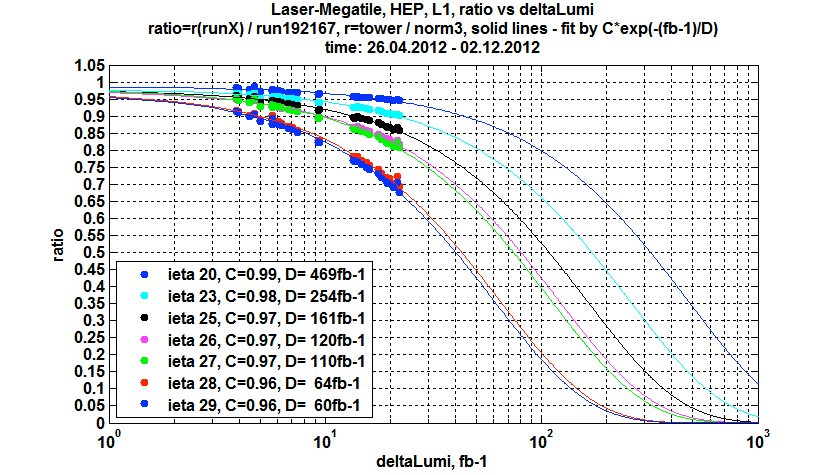
\includegraphics[width=0.49\textwidth]{figures/laserdatafits_HEP_layer1.png}
    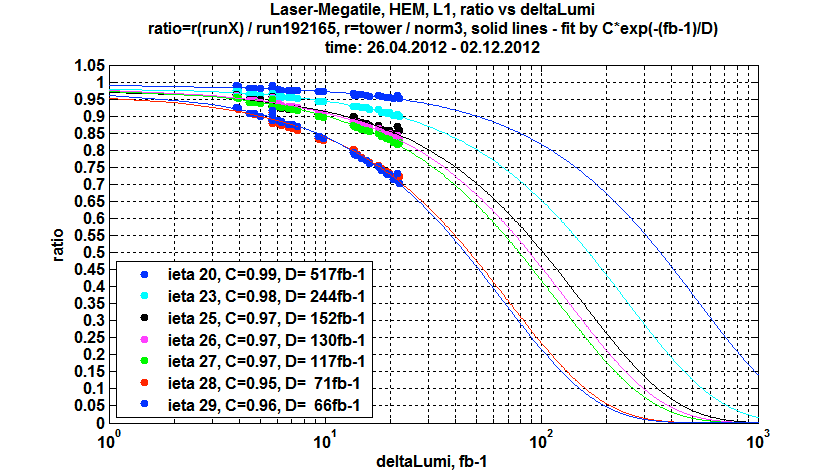
\includegraphics[width=0.49\textwidth]{figures/laserdatafits_HEM_layer1.png}
    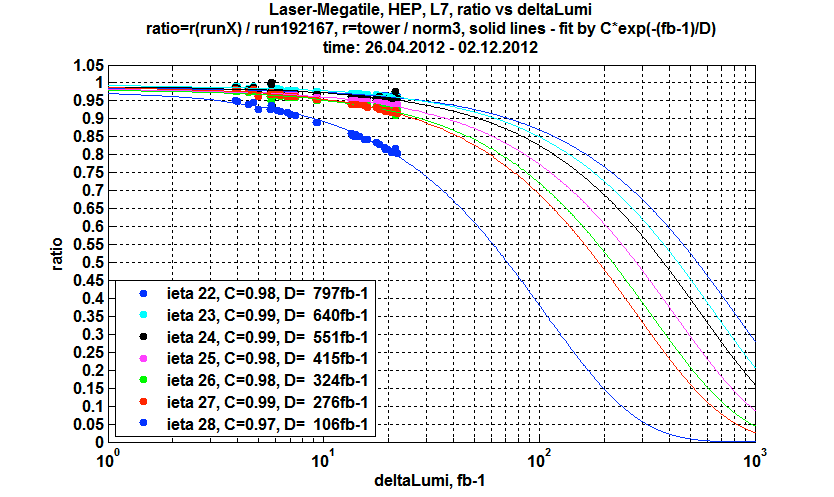
\includegraphics[width=0.49\textwidth]{figures/laserdatafits_HEP_layer7.png}
    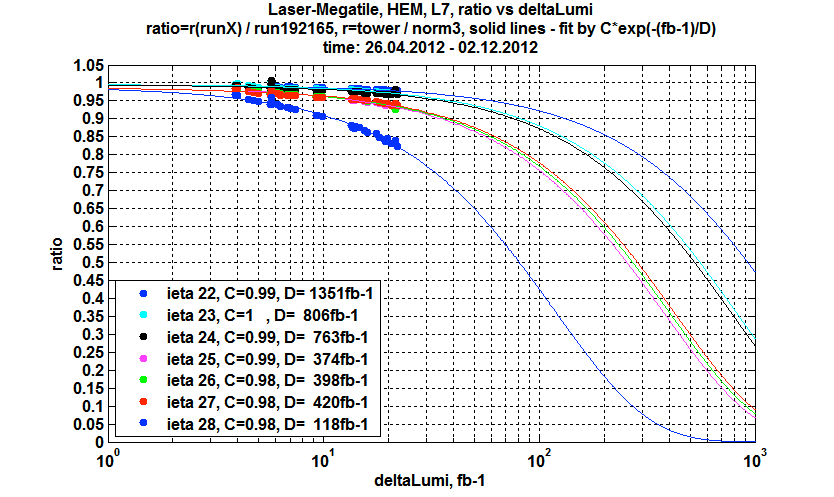
\includegraphics[width=0.49\textwidth]{figures/laserdatafits_HEM_layer7.png}
    \caption{Exponential fits to 2012 HCAL laser calibration data, for layers 1 and 7 in select towers. Data for the positive (HEP) and negative (HEM) sides of the HE are shown separately. The average of the HEP and HEM values for each scaling constant $D$ is used for the radiation damage model.~\cite{epshteyn}}
    \label{fig:laserdatafits}
  \end{center}
\end{figure}

The scaling constants from layers 1 and 7 are interpolated for layers 2-6 and extrapolated for layers 8-17, as shown in Fig. \ref{fig:laserdataconsts}.
The values from layer 1 are used for layers 0 and -1. This specifies a radiation damage model for the entire HE.
Figure \ref{fig:laserdatasignal} shows the relative signal in each layer of each tower of the HE at different integrated luminosity values, based on this radiation damage model. When the LHC center-of-mass energy increases to 14\TeV, a given integrated luminosity value will correspond to a higher amount of dose than it would at 8\TeV when the laser calibration measurements were made. To account for this, the scaling constants are divided by a factor of 1.2, based on FLUKA calculations of the difference in particle flux for 8\TeV and 14\TeV.

\begin{figure}[hbtp]
  \begin{center}
    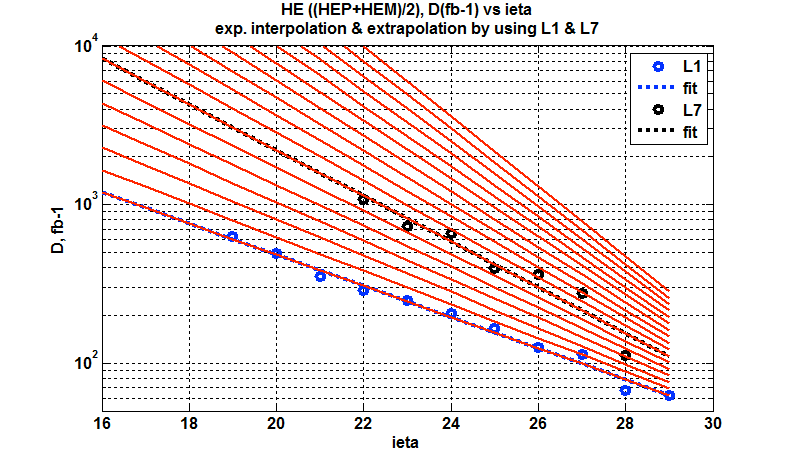
\includegraphics[width=0.98\textwidth]{figures/laserdataconsts.png}
    \caption{Interpolation and extrapolation of the scaling constants $D$ for each layer of each tower in the HE.~\cite{epshteyn}}
    \label{fig:laserdataconsts}
  \end{center}
\end{figure}

\begin{figure}[hbtp]
  \begin{center}
    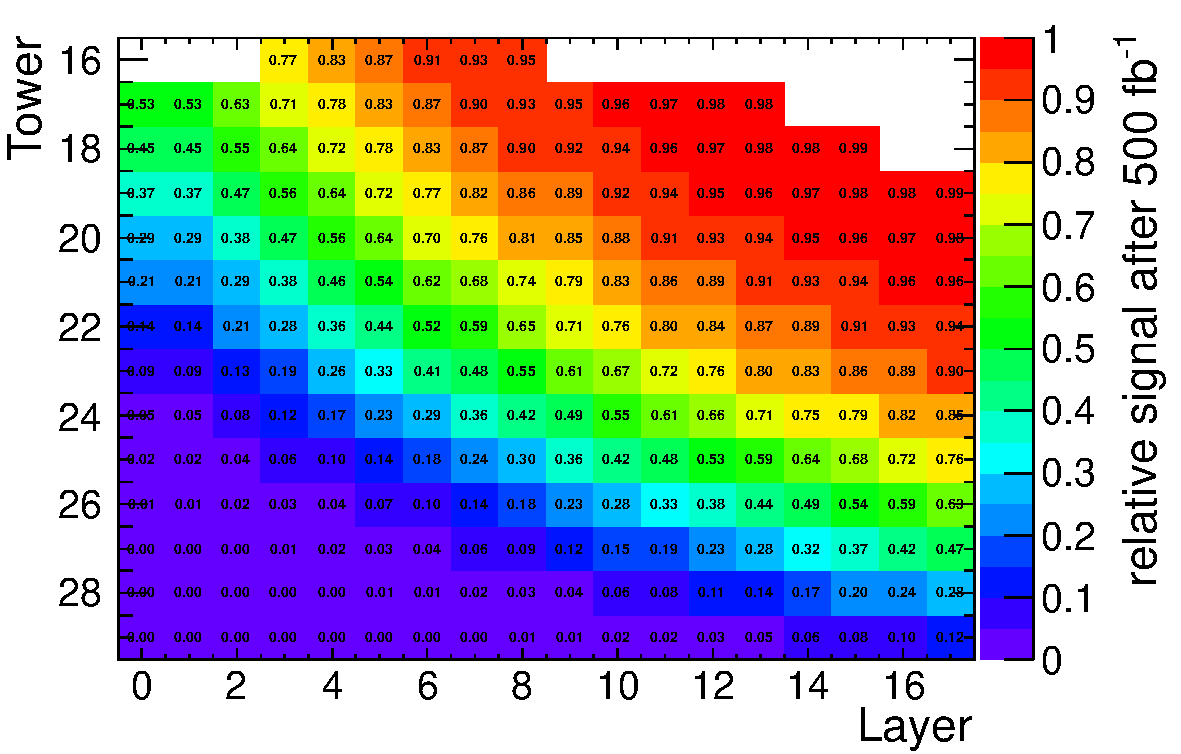
\includegraphics[width=0.98\textwidth]{figures/signal_loss_lumi500.pdf}
    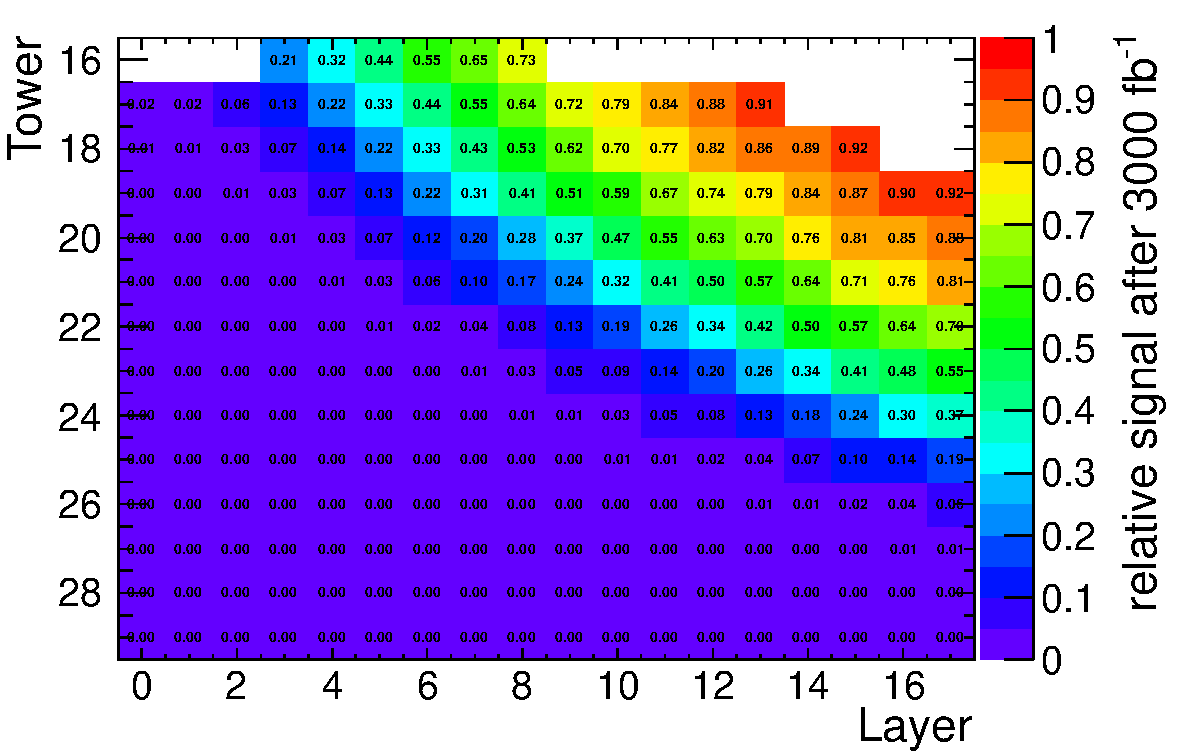
\includegraphics[width=0.98\textwidth]{figures/signal_loss_lumi3000.pdf}
    \caption{Relative signal in each layer of each tower of the HE at (a) 500\fbinv and (b) 3000\fbinv.}
    \label{fig:laserdatasignal}
  \end{center}
\end{figure}

%recalibration factors
The HE photodetectors will be recalibrated to compensate for the darkening of the scintillators and fibers. In a given tower, the light output from several layers is sent to a single photodetector. Each group of layers assigned to a photodetector in this way is called a depth. The specific arrangement of layers into depths, called the depth segmentation scheme, will be changed during the Phase 1 upgrade of the HCAL. Figure \ref{fig:hcaldepths} shows the current depth segmentation scheme and a potential upgrade scheme.

\begin{figure}[hbtp]
  \begin{center}
    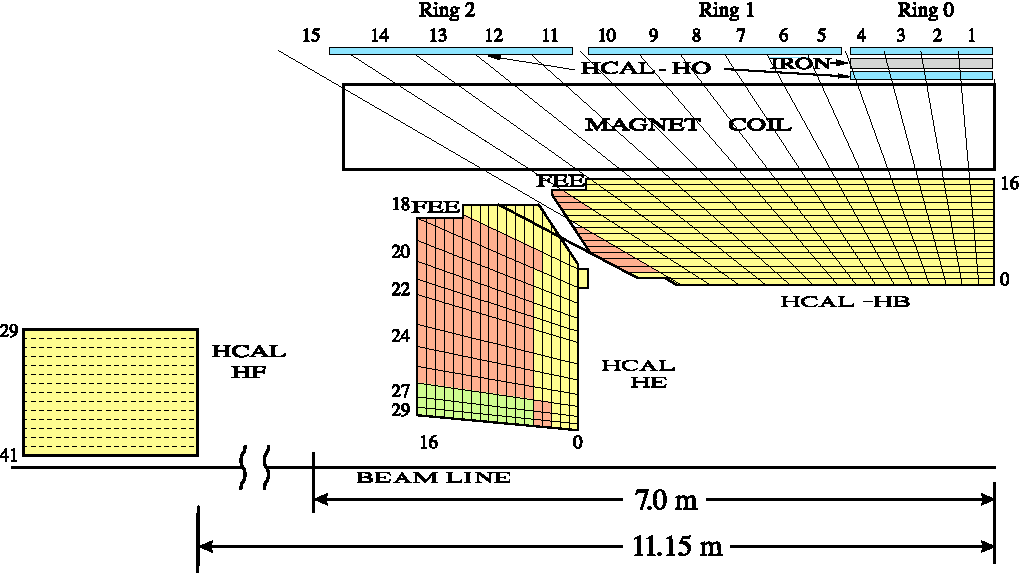
\includegraphics[width=0.49\textwidth]{figures/HCAL-HB-HE-HO-HF.pdf}
    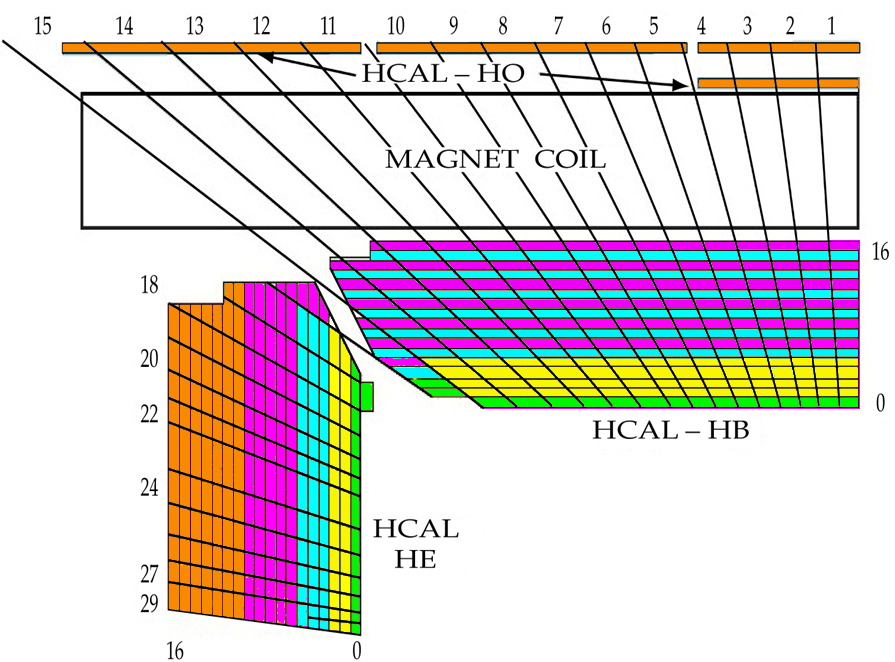
\includegraphics[width=0.49\textwidth]{figures/new_segmentation.png}
    \caption{Depth segmentation schemes in the HCAL for (a) Phase 0 with HPDs as the photodetectors and (b) a proposal for the Phase 1 upgrade with SiPMs as the photodetectors.
			Locations of the front-end electronics (FEE) for the HB and the HE are also shown.~\cite{hcaluptdr}}
    \label{fig:hcaldepths}
  \end{center}
\end{figure}

The HE radiation damage model has a specific degradation curve for each layer of each tower. This means that recalibration factors can be calculated for any depth segmentation scheme, as long as the initial relative weighting of layers within a depth is known. The weighting is determined by tabulating mean energy deposits $\langle E \rangle (\ell,i\eta,0)$ from the full simulation of 100,000 single pion events, where each pion has an energy of 50\GeV and is generated uniformly in $1.6 < \eta < 3.0$ and in $\phi$. The simulation is run at 0\fbinv, so no darkening is simulated. With these mean energy weights, the radiation damage model, and a depth segmentation scheme, recalibration factors can be calculated for any integrated luminosity:
\begin{align}
\langle E \rangle (\ell,i\eta,L) &= e^{-L/D(\ell,i\eta)}\langle E \rangle (\ell,i\eta,0) \label{eq:avgE_layer}\\
\langle E \rangle (d,i\eta,L) &= \sum_{\ell \in d} \langle E \rangle (\ell,i\eta,L) \label{eq:avgE_depth}\\
f(d,i\eta,L) &= \frac{\langle E \rangle (d,i\eta,0)}{\langle E \rangle (d,i\eta,L)} \label{eq:factor_depth}
\end{align}

Equation \eqref{eq:avgE_layer} shows how to use the radiation damage model to find the weights at a given integrated luminosity value, based on the weights at 0\fbinv. Equation \eqref{eq:avgE_depth} is a sum of the weights for the layers in a given depth, determined by the depth segmentation scheme. Equation \eqref{eq:factor_depth} gives the calculation for the recalibration factor at a given depth and integrated luminosity. In these equations, $\langle E \rangle$ is the average energy used as a weight (for layers or for depths), $\ell$ is the layer number, $i\eta$ is the tower number, $L$ is the integrated luminosity in \fbinv, $d$ is the depth number, and $f$ is the recalibration factor.

The recalibration factors for the specified Phase 0 and Phase 1 depth segmentation schemes are shown in Figs. \ref{fig:recalib_phase0} and \ref{fig:recalib_phase1}, respectively. In practice, a maximum recalibration cutoff will be assigned so that photodetector signals and noise are not multiplied by absurdly large values. The default cutoff values are 20 for HPDs and 100 for SiPMs, shown on the figures. %reference the optimization of cutoff values here?

\begin{figure}[hbtp]
  \begin{center}
    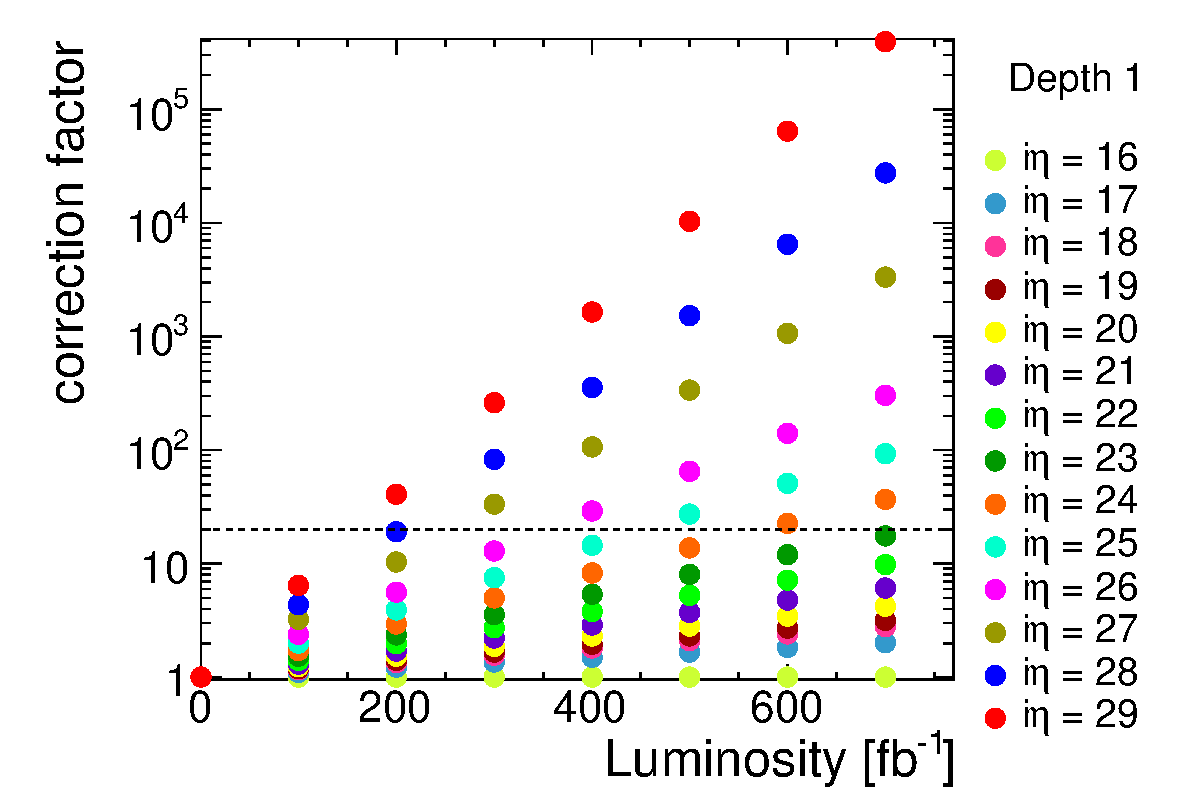
\includegraphics[width=0.49\textwidth]{figures/mean_corr_comp_depth_1_phase0.pdf}
    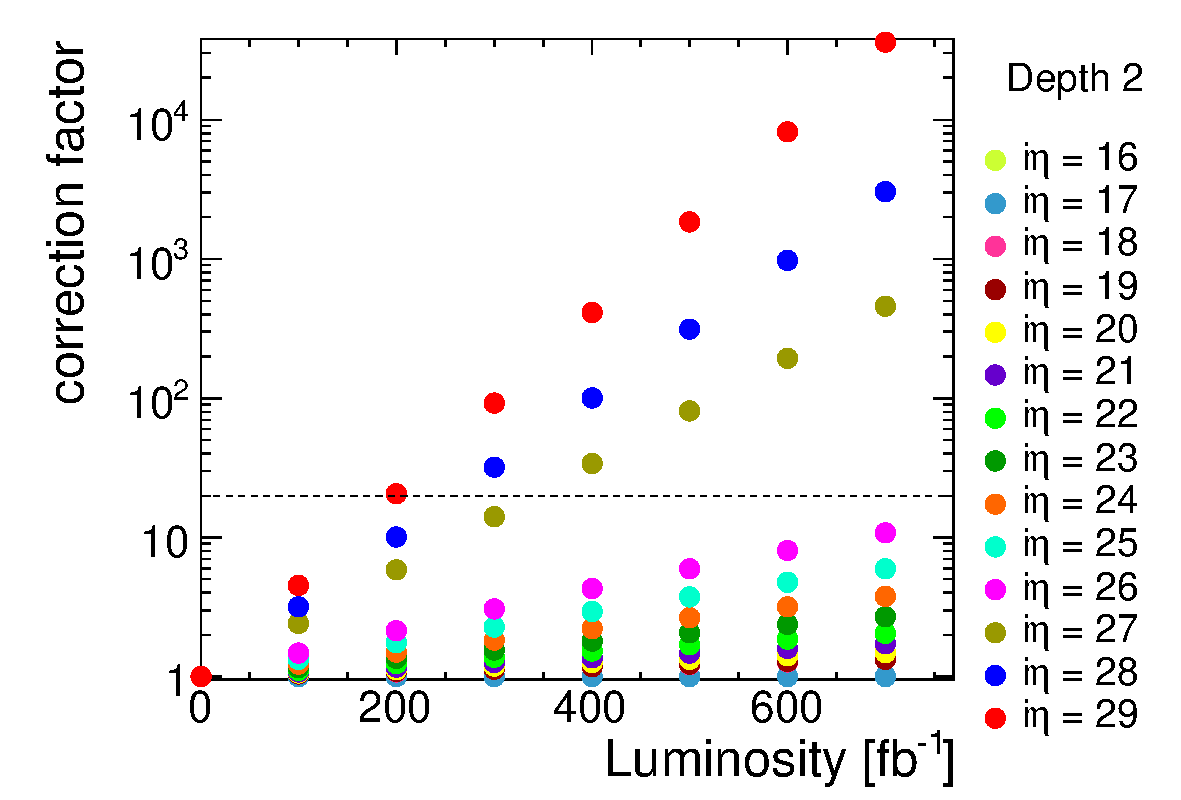
\includegraphics[width=0.49\textwidth]{figures/mean_corr_comp_depth_2_phase0.pdf}
    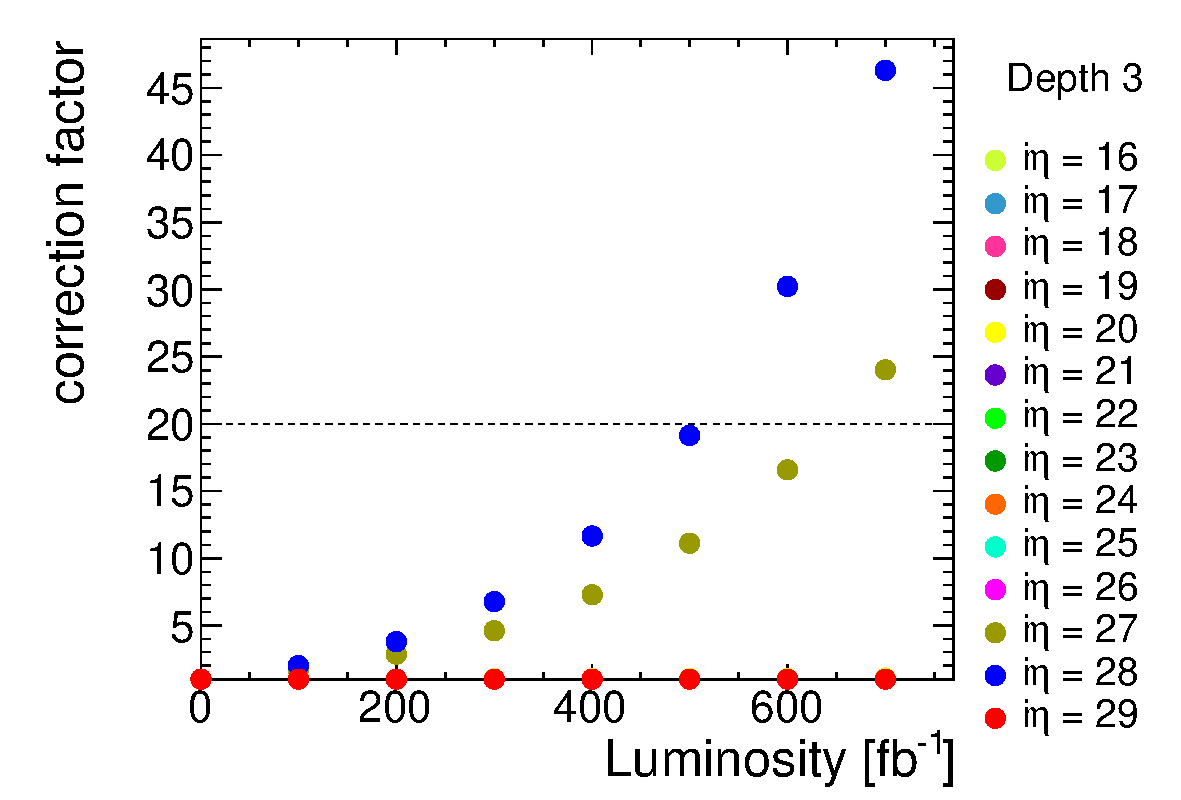
\includegraphics[width=0.49\textwidth]{figures/mean_corr_comp_depth_3_phase0.pdf}
    \caption{Recalibration factors for the Phase 0 depth segmentation scheme. The default recalibration cutoff of 20 is shown as a dotted line on each plot.}
    \label{fig:recalib_phase0}
  \end{center}
\end{figure}

\begin{figure}[hbtp]
  \begin{center}
    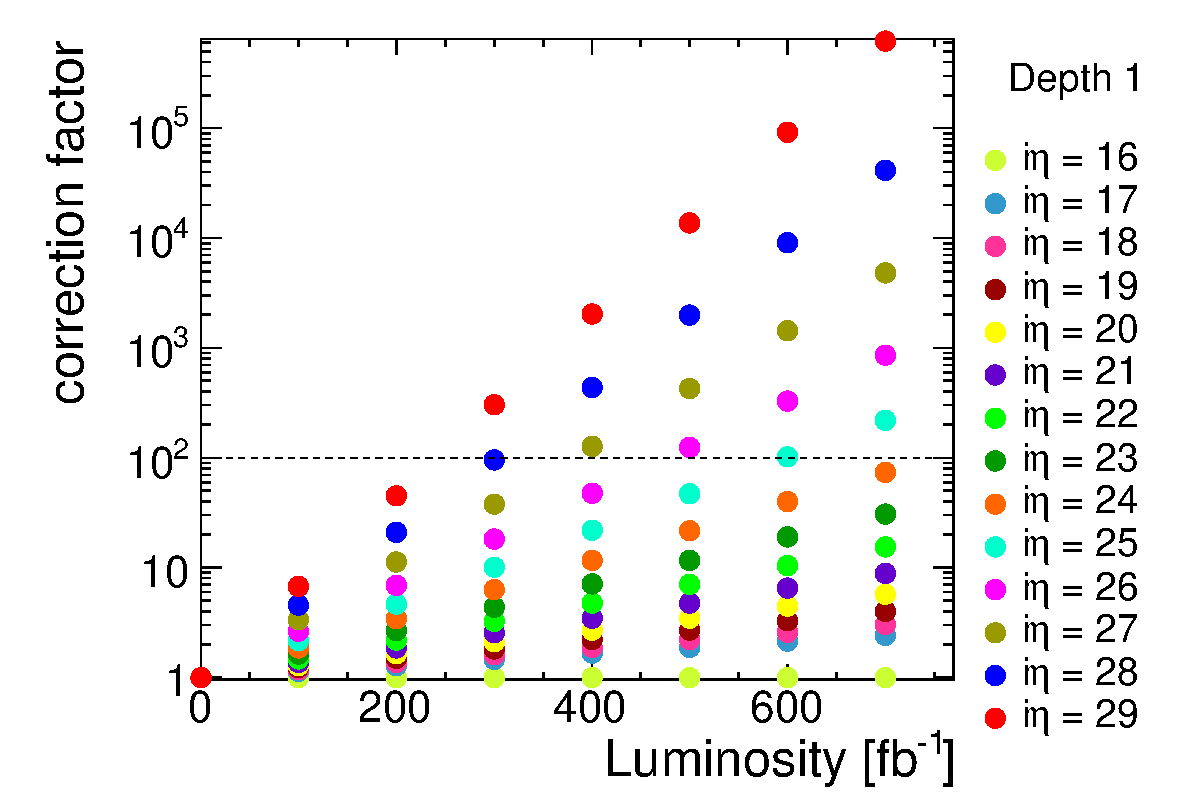
\includegraphics[width=0.49\textwidth]{figures/mean_corr_comp_depth_1_zoom.pdf}
    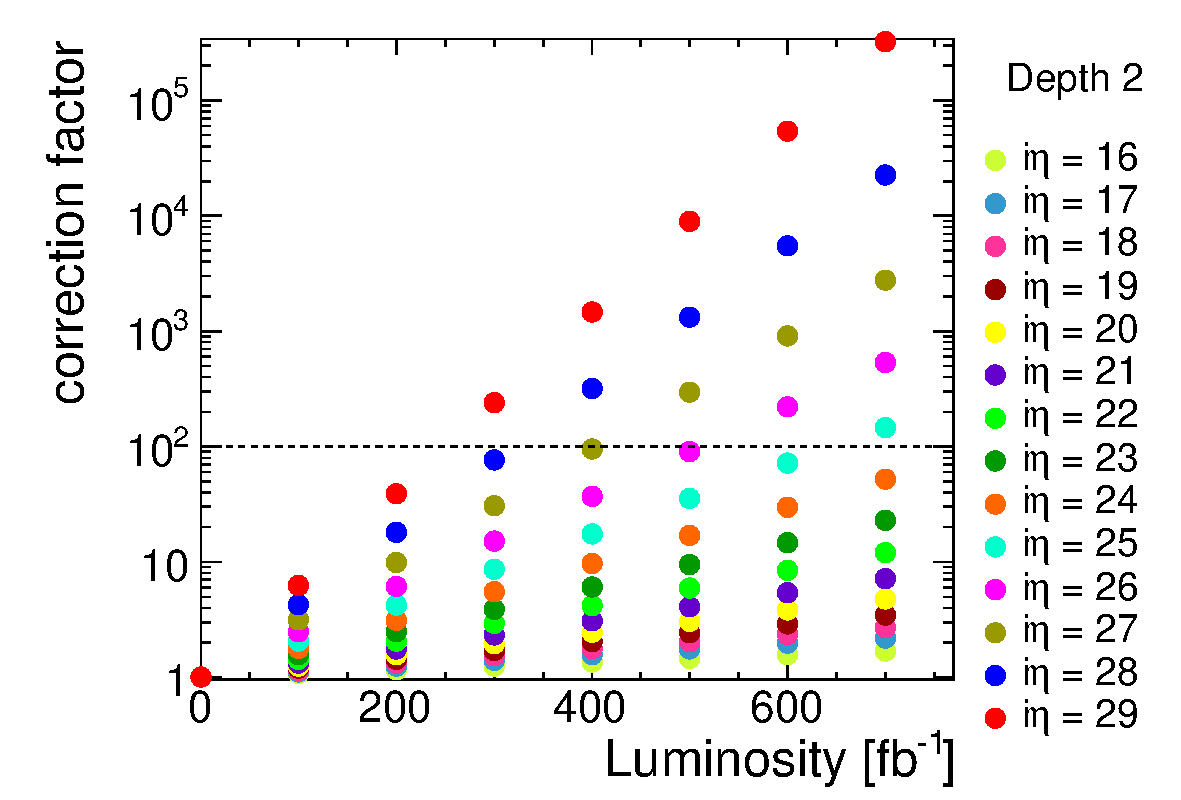
\includegraphics[width=0.49\textwidth]{figures/mean_corr_comp_depth_2_zoom.pdf}
    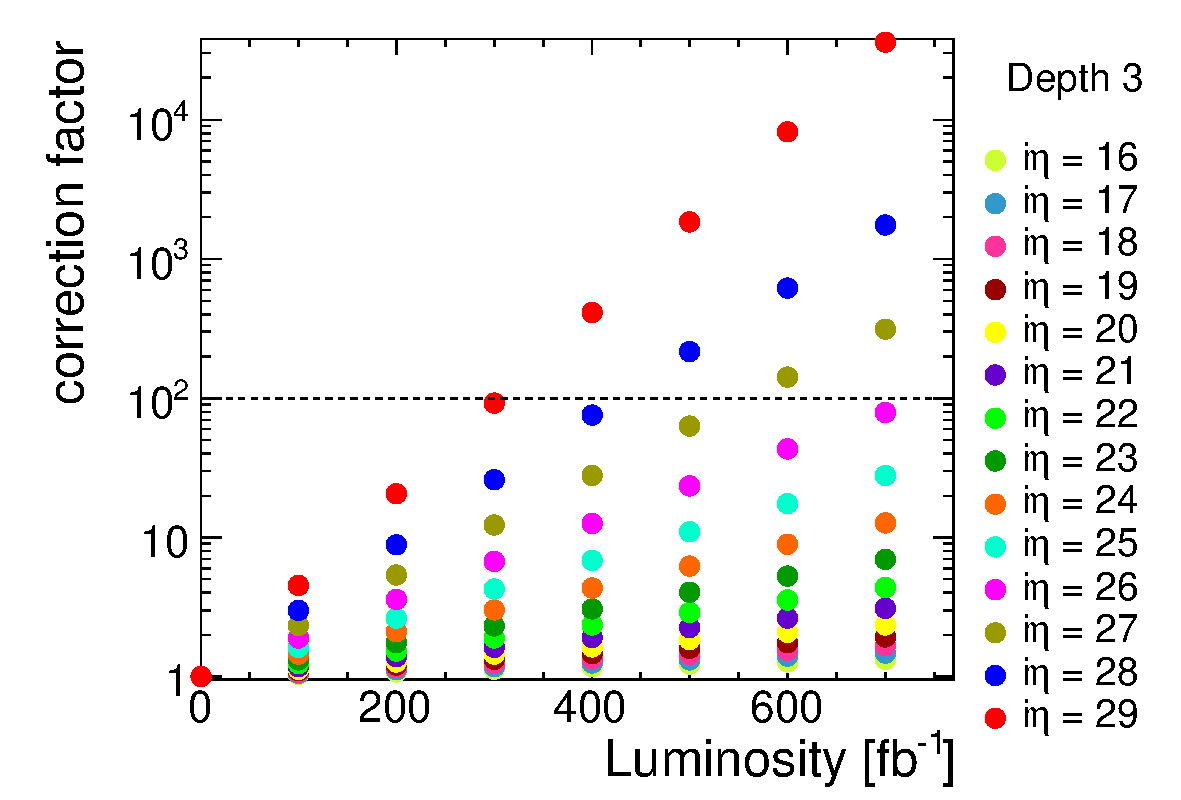
\includegraphics[width=0.49\textwidth]{figures/mean_corr_comp_depth_3_zoom.pdf}
    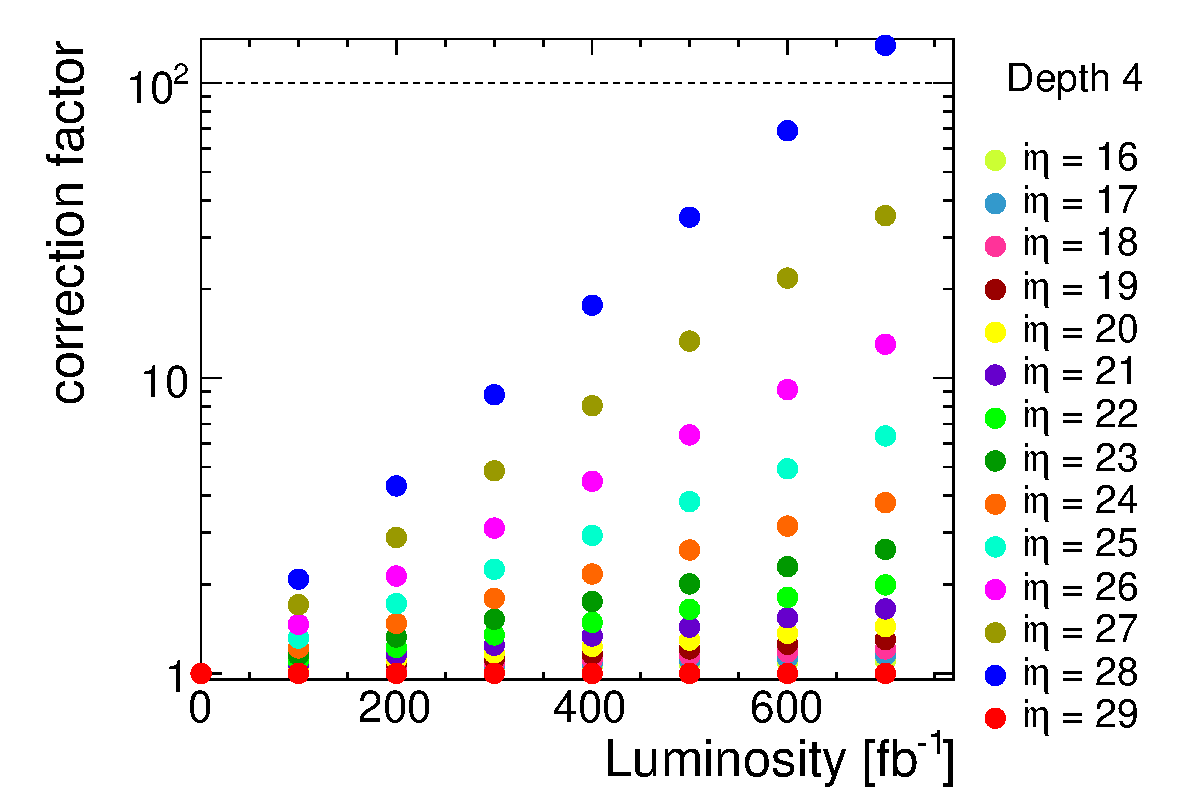
\includegraphics[width=0.49\textwidth]{figures/mean_corr_comp_depth_4_zoom.pdf}
    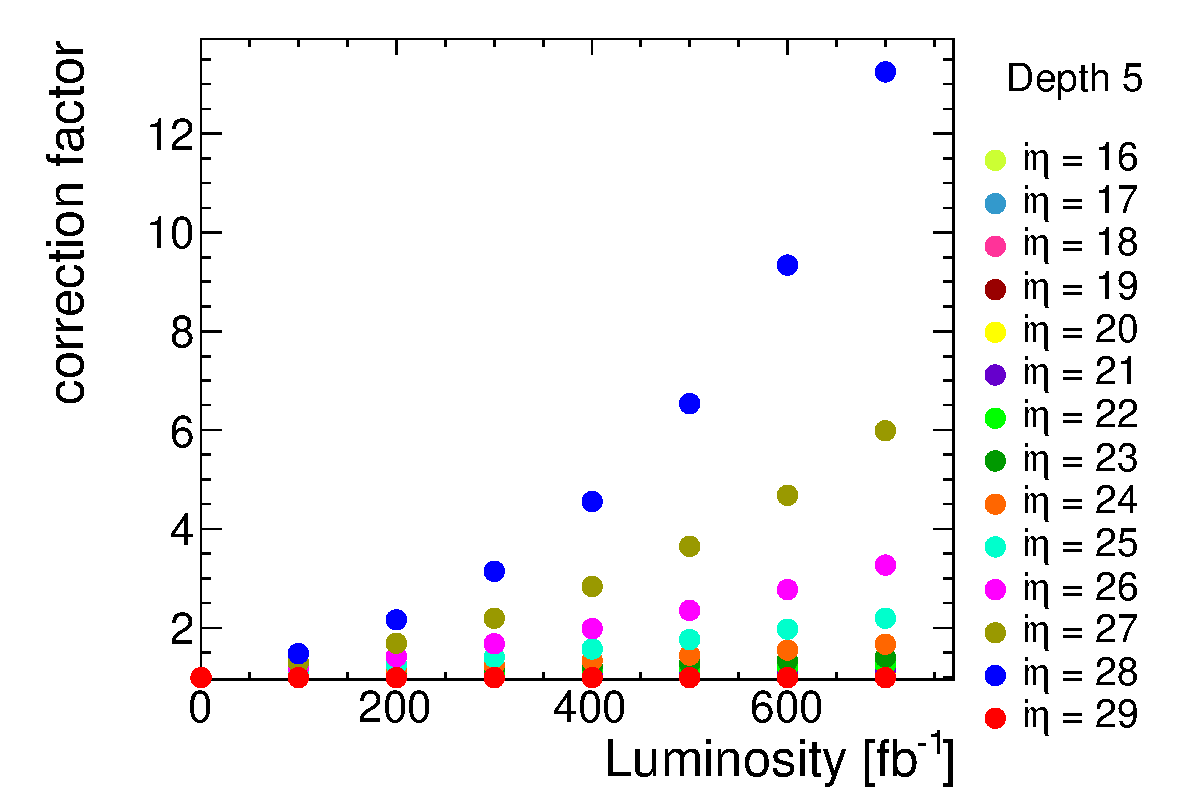
\includegraphics[width=0.49\textwidth]{figures/mean_corr_comp_depth_5_zoom.pdf}
    \caption{Recalibration factors for the proposed Phase 1 depth segmentation scheme. The default recalibration cutoff of 100 is shown as a dotted line on each plot.}
    \label{fig:recalib_phase1}
  \end{center}
\end{figure}

%sipm pedestal widths
Radiation does not have a large effect on the pedestal widths of the HPDs. However, the SIPMs' dark current grows with increasing radiation dose, which leads photodetector noise to increase with integrated luminosity. The simulation of SiPMs accounts for these luminosity-dependent pedestal widths with the following equations, based on measurements shown in Fig. \ref{fig:sipm_darkcurrent}:
\begin{align}
L_{\text{eff}} &= \text{max}(L - 200\fbinv,0) \label{eq:Leff} \\
\sigma_{\text{SiPM}}^{\text{(HB)}} &= 5 + 1.7 \sqrt{L_{\text{eff}}}~\text{[fC]} \label{eq:sipmwidthHB}\\
\sigma_{\text{SiPM}}^{\text{(HE)}} &= 5 + 0.7 \sqrt{L_{\text{eff}}}~\text{[fC]} \label{eq:sipmwidthHE}
\end{align}

Equation \eqref{eq:Leff} accounts for the planned installation of the SiPMs after 200\fbinv have already been collected. Equations \eqref{eq:sipmwidthHB} and \eqref{eq:sipmwidthHE} show the scaling of the pedestal widths with the square root of integrated luminosity. The increase in dark current also changes the pedestal means and zero suppression thresholds, and the simulation accounts for these changes.

\begin{figure}[hbtp]
  \begin{center}
    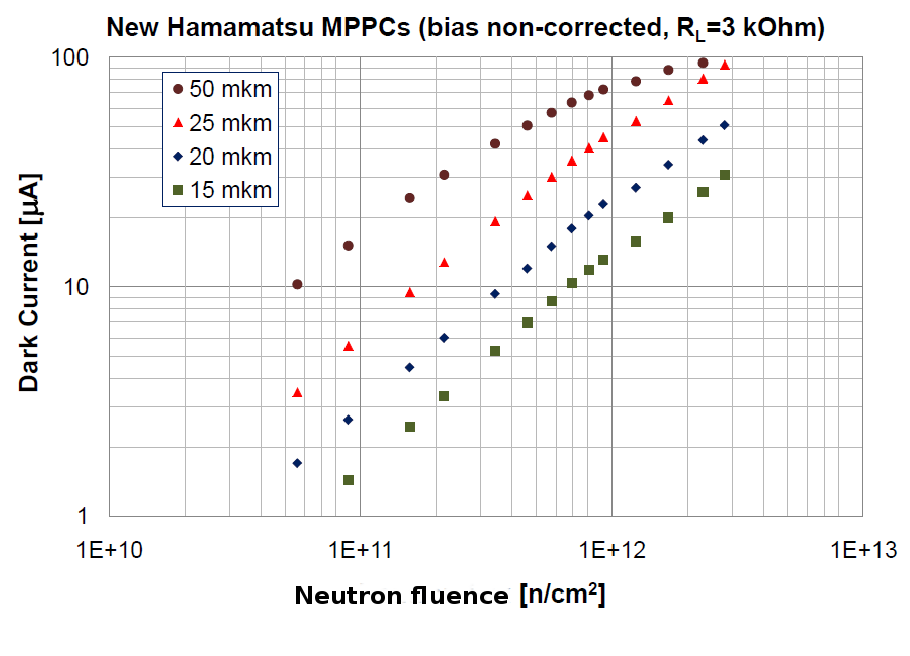
\includegraphics[width=0.98\textwidth]{figures/leakagecurrentneutrons.png}
    \caption{Plot of the SiPM dark current for different radiation doses.~\cite{hcaluptdr}}
    \label{fig:sipm_darkcurrent}
  \end{center}
\end{figure}

\subsection{Jet Studies with Radiation Damage}

\section{Phase 2 Simulations}

\subsection{Validation of Upgrade Standalone Simulation}
\label{sec:newdetval}

In order to simulate different options for new calorimeters, the FCAL Task Force created a standalone Geant4 simulation with a simplified geometry based on the CMS endcap detector specifications as given in Ref.~\cite{cmsatcern}. The simulation geometry uses the same coordinate system as the real CMS geometry, with $z$ as the beamline and $x, y$ as the transverse directions. The detector components all have the shape of rectangular prisms with transverse dimensions $540\unit{cm} \times 540\unit{cm}$. The preshower is simulated as 3\unit{cm} of aluminum, 1.5\unit{cm} of lead, and a G10 cryogenic plate. The EE is constructed as a 22\unit{cm} deep homogeneous medium of $\text{PbWO}_{4}$. Between the EE and the HE, there is a section of dead material, which is modeled as 23.4\unit{cm} of a mixture of copper and polymer to simulate cables. The HE is 149.6\unit{cm} deep with 17 sampling layers, each consisting of 79\unit{mm} brass, 3.7\unit{mm} plastic scintillator, air gaps, and aluminum shielding. At the front of the HE there is a 15\unit{mm} zero layer, including 9\unit{mm} plastic scintillator, air gaps, and aluminum shielding. Energy deposits in the zero layer are weighted with a factor of 0.5 to account for its larger size.  Figure \ref{fig:showers} shows a side view of the simulated geometry with particle showers propagating through the calorimeters.

%figure: standalone showers
\begin{figure}[hbtp]
\begin{center}
%placeholder (filesize)
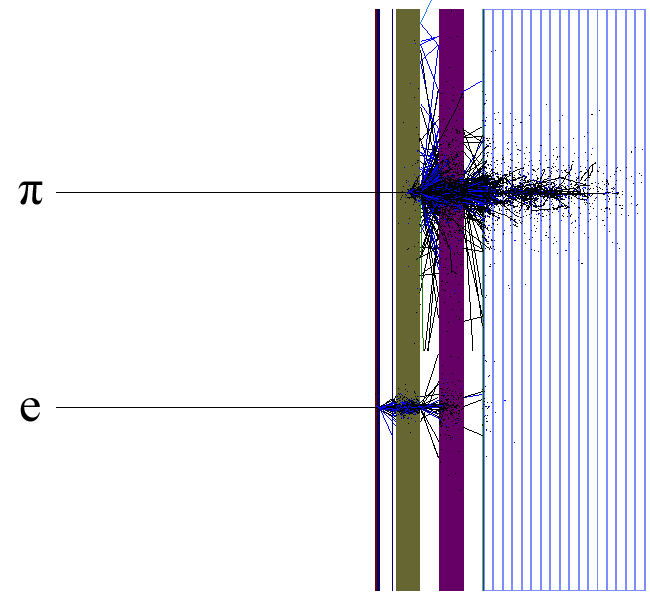
\includegraphics[width=0.75\textwidth]{figures/showers-labeled.png}
\caption{Geant4 visualization of the standalone simulation with particle showers from a 500\GeV pion (top) and 500\GeV electron (bottom). From left to right: preshower (dark blue), EE (gold), dead material (purple), HE (blue and white).}
\label{fig:showers}
\end{center}
\end{figure}

To ensure that the essential physics and detector behavior are present in the standalone simulation, it was validated against the CMSSW full simulation using pions and the settings given in Sec. \ref{sec:newdetvalcmssw}. The validation compared the pion response and resolution from SimHits, since the standalone simulation does not include a simulation of electronics or event reconstruction. Several subtle effects and details had to be taken into account in order to reproduce the CMSSW full simulation results in the standalone simulation.

\subsubsection{Sampling Factors}
\label{sec:newdetvalsam}

The HCAL is a sampling calorimeter which collects only a fraction of the total energy of incident particles. A conversion factor is needed to estimate how the collected energy corresponds to the original particle's energy. There are numerous methods for calculating this sampling factor, and variations in it can lead to significant differences in energy response. To ensure similarity to the CMSSW full simulation, the sampling factor algorithm for the standalone simulation follows the CMSSW algorithm, described in Ref.~\cite{hcalsam}, as closely as possible. The simplified geometry of the standalone simulation means that there is no structure of $i\eta$ towers and therefore no need to iterate the algorithm to account for the spread of energy over different towers.

Sampling factors are calculated by selecting from a sample of 50\GeV pions only the pions which act as minimum ionizing particles (mips) in the ECAL, so each shower is largely contained within the HCAL and a comparison to the incident energy of 50\GeV is appropriate. Based on the energy distribution of pions in the ECAL, a mip threshold of $E_{\text{ecal}} < 1\GeV$ was chosen. The sampling factor is calculated from a sample of pions which pass this threshold:
\begin{equation} \label{fsam} f_{\text{hcal}} = \frac{E_{\text{gen}}}{E_{\text{hcal}}^{*}}\,, \end{equation}
where $E_{\text{hcal}}^{*}$ is the peak, or most probable, energy deposited in the HCAL from that pion sample. Applying Eq. \eqref{fsam} to both the standalone simulation and the CMSSW full simulation, with settings which will be specified below, gives values $f_{\text{hcal}}^{\text{standalone}} = 178$ and $f_{\text{hcal}}^{\text{CMSSW}} = 183$, showing good agreement.

\subsubsection{Birks' Law for the Electromagnetic Calorimeter}
\label{sec:newdetvalbirks}

Organic scintillators have a nonlinear energy response due to quenching. Birks' Law \cite{birks} describes this nonlinearity with several parameterizations comparing the scintillator light output to the energy deposited by a particle. Inorganic scintillators, too, may have a nonlinear energy response, which requires a different parameterization. During the development of the CMSSW full simulation, it was found that the agreement of simulation with data for the ECAL improved when using the parameterization developed for the BGO detector at the L3 experiment~\cite{datadriven}. The BGO values must be used directly, as the nonlinearity of $\text{PbWO}_{4}$ has not been measured. This parameterization has also been included in the standalone simulation:
\begin{align}
\label{ecalbirks} \frac{dL}{dr} &= w\frac{dE}{dr}\,, \\
\label{ecalbirksw} w &= 1 - s \cdot \text{log}\left(k\frac{dE}{dr}\right)\,,
\end{align}
where $dL/dr$ is the light output, $dE/dr$ is the energy deposited, and $w$ is the weight factor which introduces the nonlinearity. The parameter $s$ is an empirical slope factor, and $k$ is related to Birks' constant $kB$. After $w$ is calculated in Eq. \eqref{ecalbirksw}, its bounds are checked: if it is lower than a parameter $c$, it is set equal to $c$; if it is higher than 1, it is set equal to 1. The BGO values of these parameters, which are applied to $\text{PbWO}_{4}$, are $k = 0.03333$, $s = 0.253694$, and $c = 0.1$.

\subsubsection{Dead Material}
\label{sec:newdetvaldead}

Initial versions of the standalone geometry included only a small amount, 1.5\unit{mm}, of dead material between the ECAL and the HCAL. However, in the real detector there is a much larger amount of dead material, consisting of cables, support structures, and cooling systems. Using the material budget tool described in Ref.~\cite{matbudget}, the CMSSW full simulation geometry was scanned at $\eta = 2$, roughly the center of the endcap, for various $\phi$ values. The depths of all materials between the end of the ECAL crystals and the start of the HCAL structure are summed to find a range of dead material varying in $\phi$ between 0.57 $\lambda_{0}$ and 0.63 $\lambda_{0}$. Geant4 has an internal formula for the nuclear interaction length, which calculated $\lambda_{0} = 389.98\unit{mm}$ for the copper-polymer material used to simulate the dead material. The depth of this material was increased to $234\unit{mm} = 0.6~\lambda_{0}$, the average of the scanned material budget range, and the volume was placed to be centered between the ECAL and the HCAL as depicted in Fig. \ref{fig:showers}.

\subsubsection{CMSSW Settings}
\label{sec:newdetvalcmssw}

There are several settings in the CMSSW full simulation which can be modified to increase the similarity with the standalone simulation. A calorimeter-only geometry was selected in order to remove the tracker, which is not included in the standalone simulation. The magnetic field was turned off; though a magnetic field could instead be turned on in the standalone simulation, turning off the field prevents lower-energy particles from being deflected away from the center of the endcap, $\eta = 2$, where the CMSSW calorimeter geometry most closely resembles the standalone geometry. Finally, by default CMSSW uses a customized physics list QGSP\_FTFP\_BERT\_EML \cite{calotf}, which was changed to the standard QGSP\_BERT\_EMV to match the standalone simulation.

\subsubsection{Pion Results}
\label{sec:newdetvalres}

Using the sampling factors given in Sec. \ref{sec:newdetvalsam}, reconstructed energies for pions are calculated as:
\begin{equation} \label{Erec} E_{\text{rec}} = E_{\text{ecal}} + f_{\text{hcal}} \cdot E_{\text{hcal}}\,. \end{equation}
Energy response and resolution are calculated from a Gaussian fit based on the mean $m$ and standard deviation $s$ of the energy distributions, over a range $[m-2s, m+s]$ to account for the high tail. Figure \ref{fig:valfits} shows example energy distributions and fits for 50\GeV pions, and Fig. \ref{fig:valbanana} shows two-dimensional plots of the ECAL energy vs. the HCAL energy. Both figures show good agreement between the standalone simulation and the CMSSW full simulation. This agreement extends over a large range of pion energies, 1\GeV to 3\TeV, as demonstrated in Fig. \ref{fig:valplots}.

%figure: pion fit example
\begin{figure}[hbtp]
\begin{center}
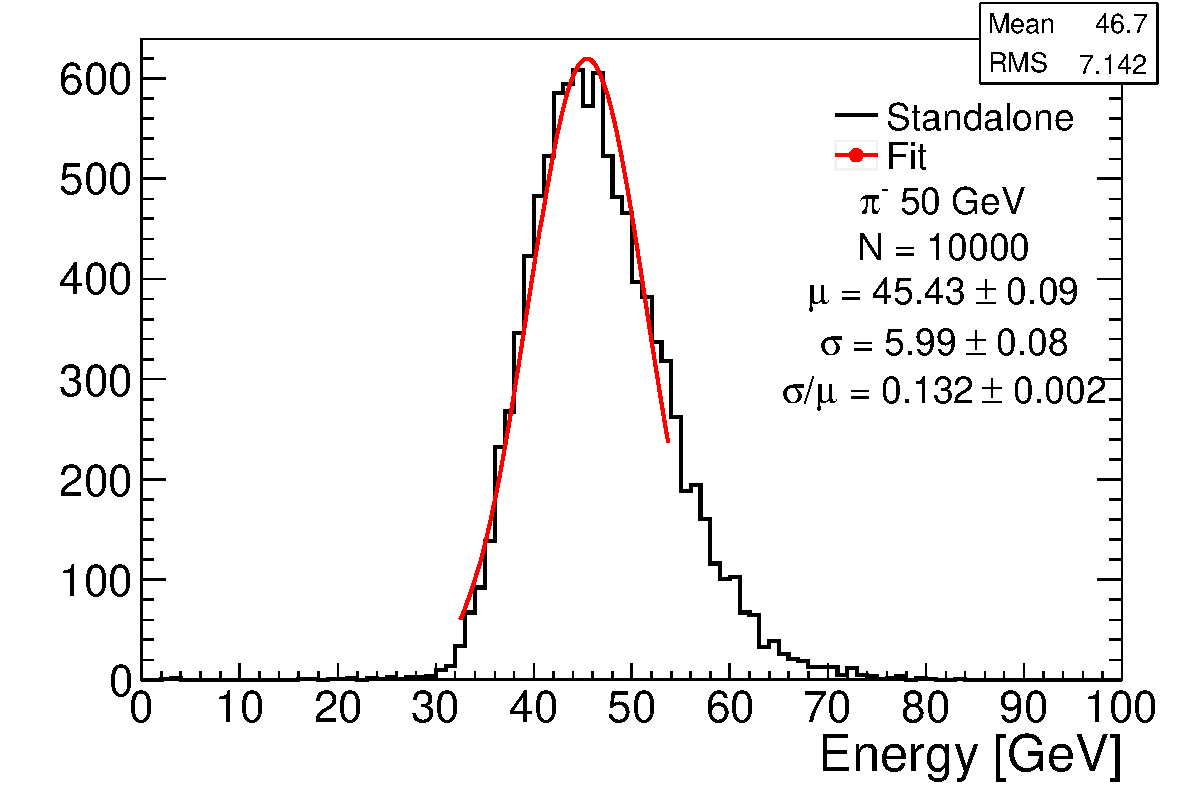
\includegraphics[width=0.49\textwidth]{figures/g4_hcal_tot_res_fit_50gev.pdf}
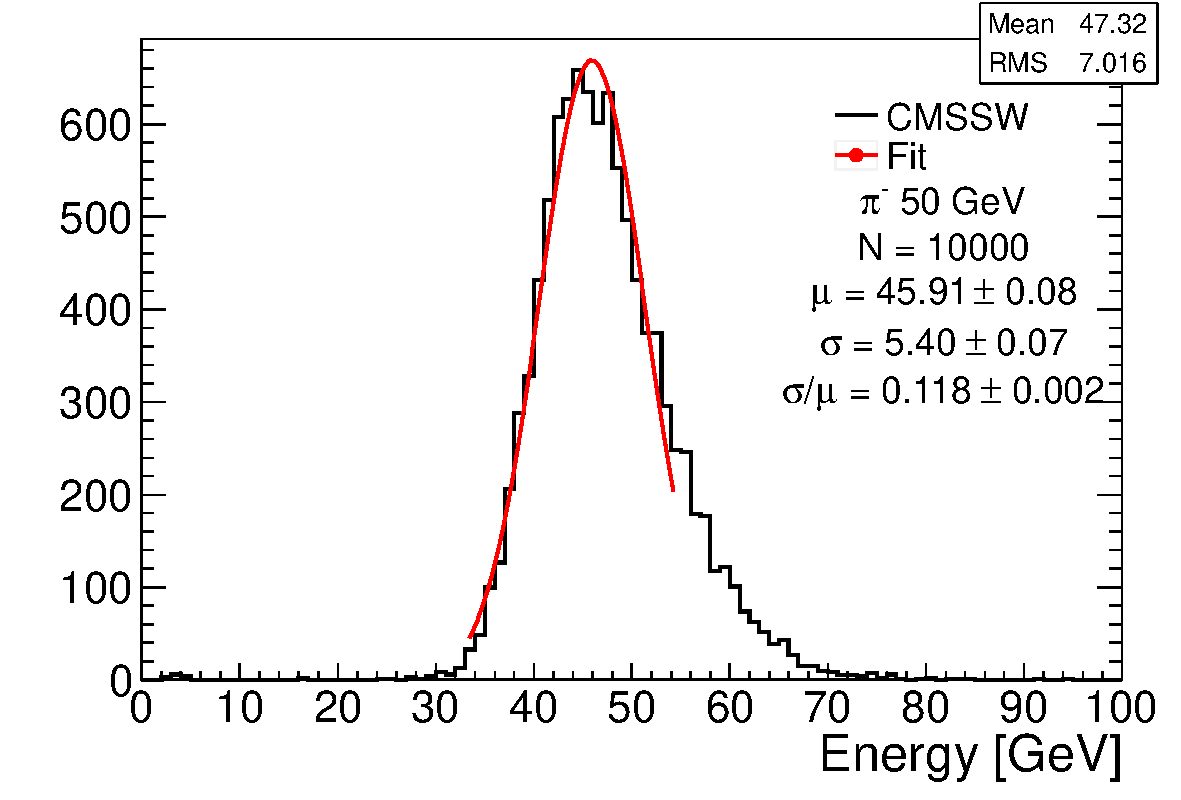
\includegraphics[width=0.49\textwidth]{figures/fs_hcal_tot_res_fit_50gev.pdf}
\caption{Energy distributions from 10\,000 pions at 50\GeV, fit with Gaussians, for the standalone simulation (left) and the CMSSW full simulation (right).}
\label{fig:valfits}
\end{center}
\end{figure}

%figure: pion banana plots
\begin{figure}[hbtp]
\begin{center}
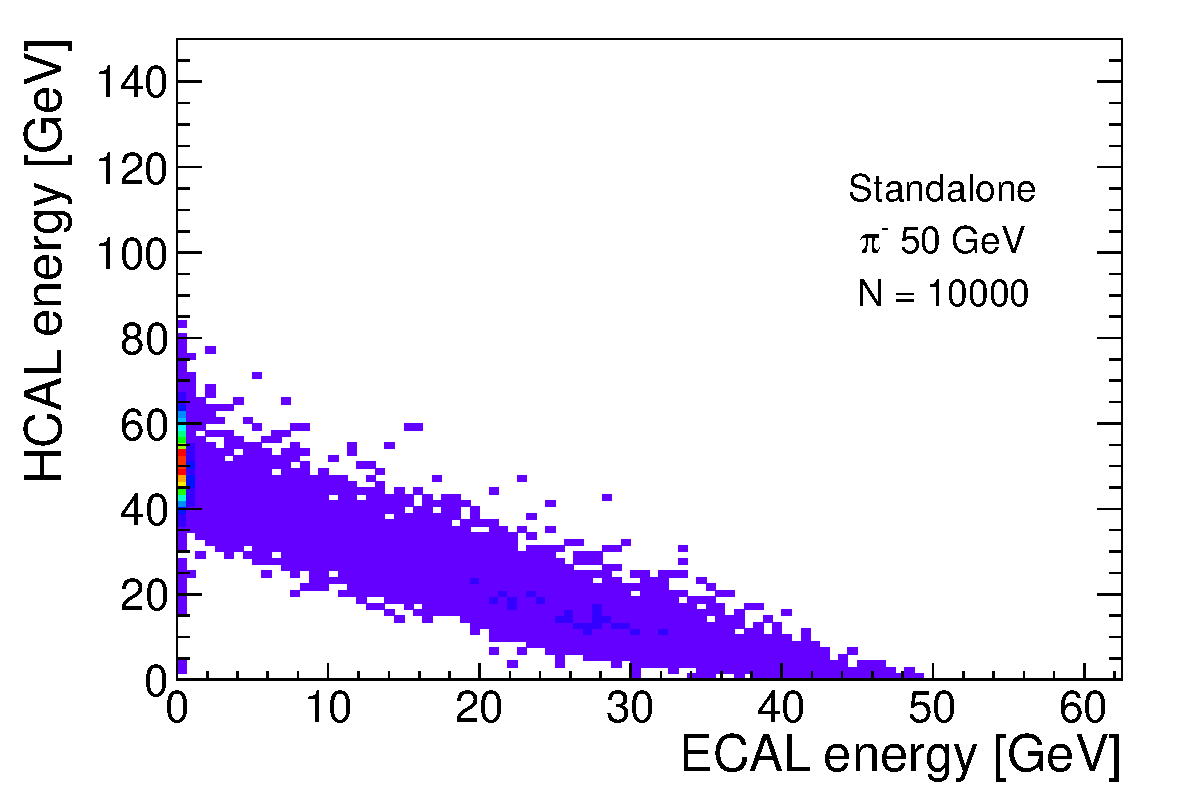
\includegraphics[width=0.49\textwidth]{figures/g4_banana_plot_tot_50gev.pdf}
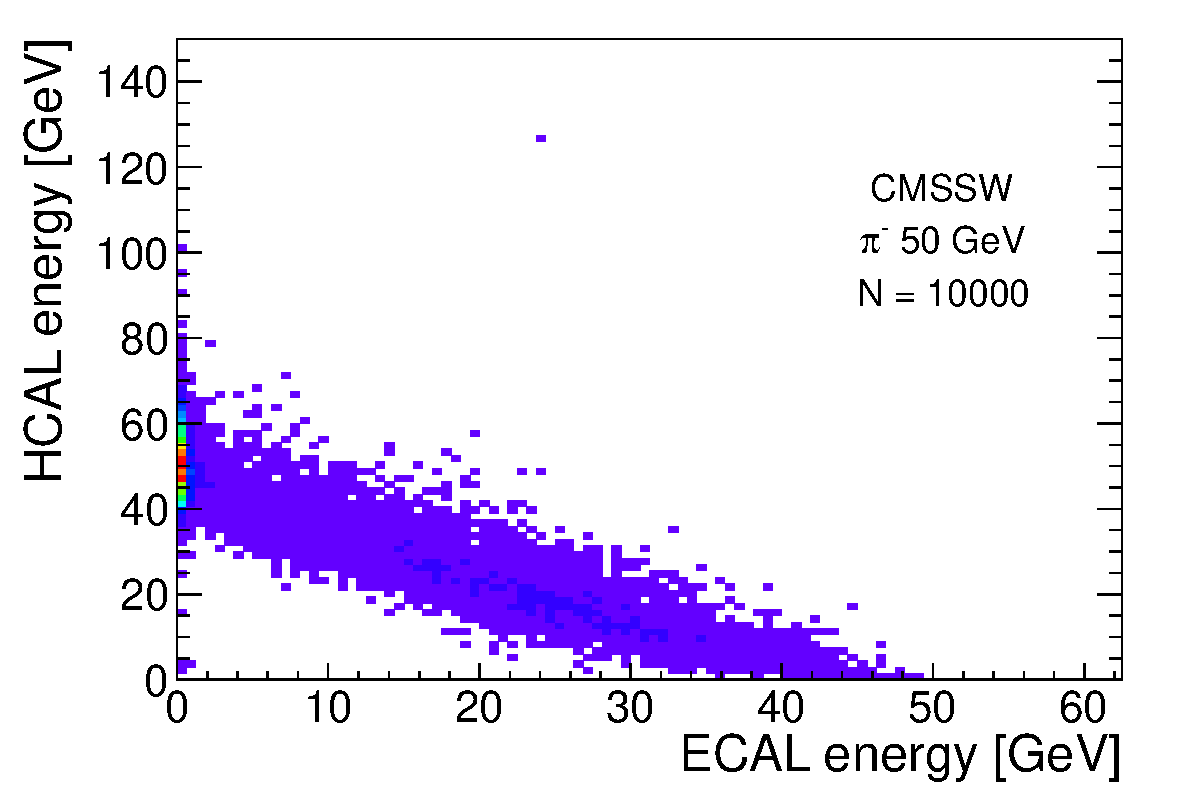
\includegraphics[width=0.49\textwidth]{figures/fs_banana_plot_tot_50gev.pdf}
\caption{The ECAL energy vs. the HCAL energy from 10\,000 pions at 50\GeV, for the standalone simulation (left) and the CMSSW full simulation (right).}
\label{fig:valbanana}
\end{center}
\end{figure}

%figure: pion validation plots
\begin{figure}[hbtp]
\begin{center}
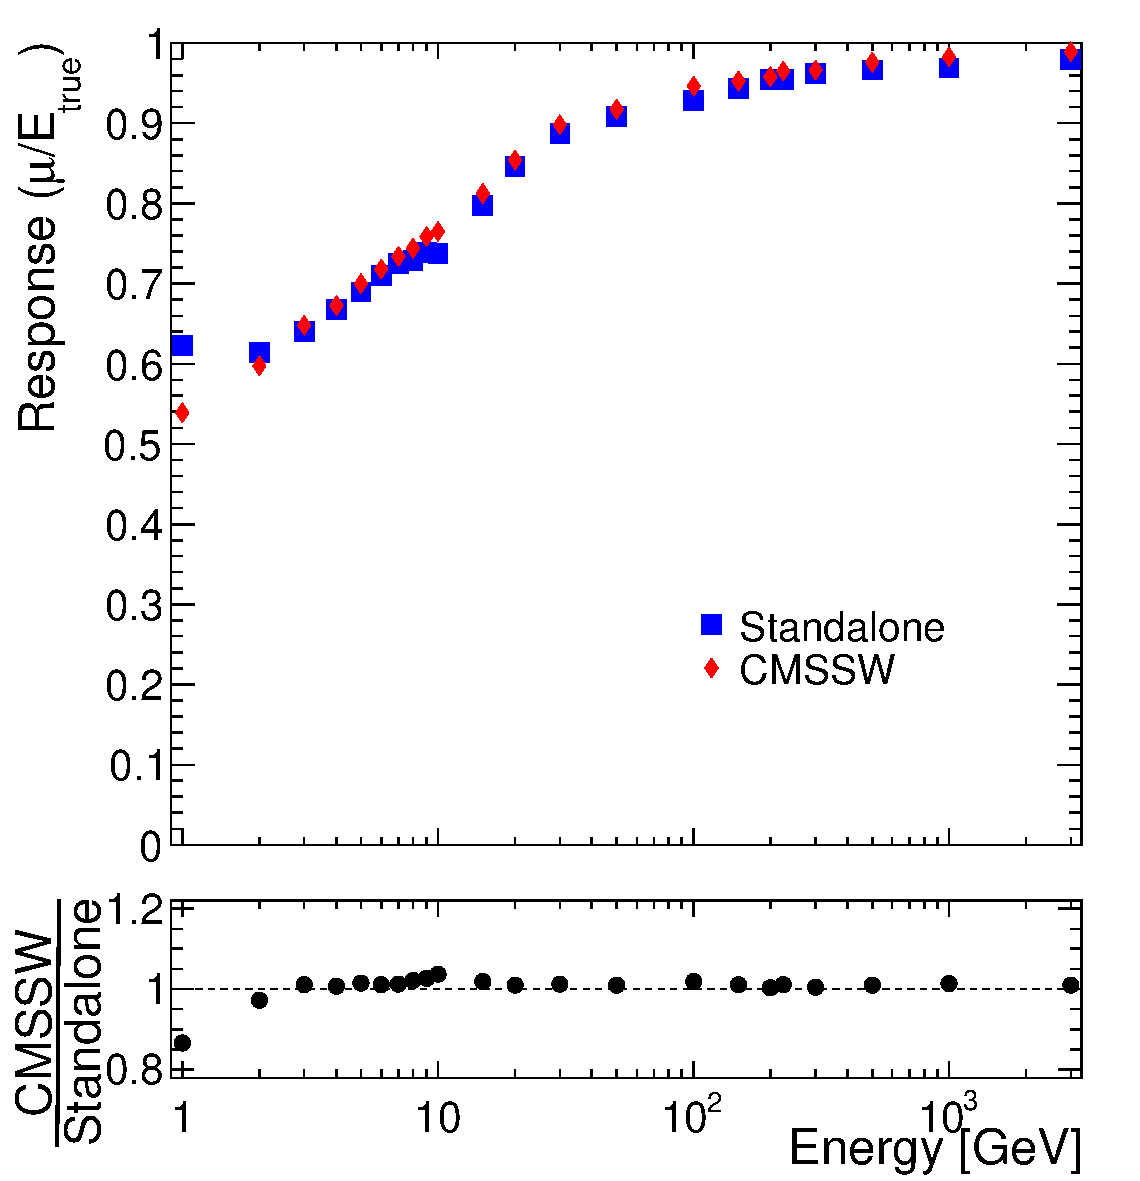
\includegraphics[width=0.49\textwidth]{figures/hcal_mu_comp_tot.pdf}
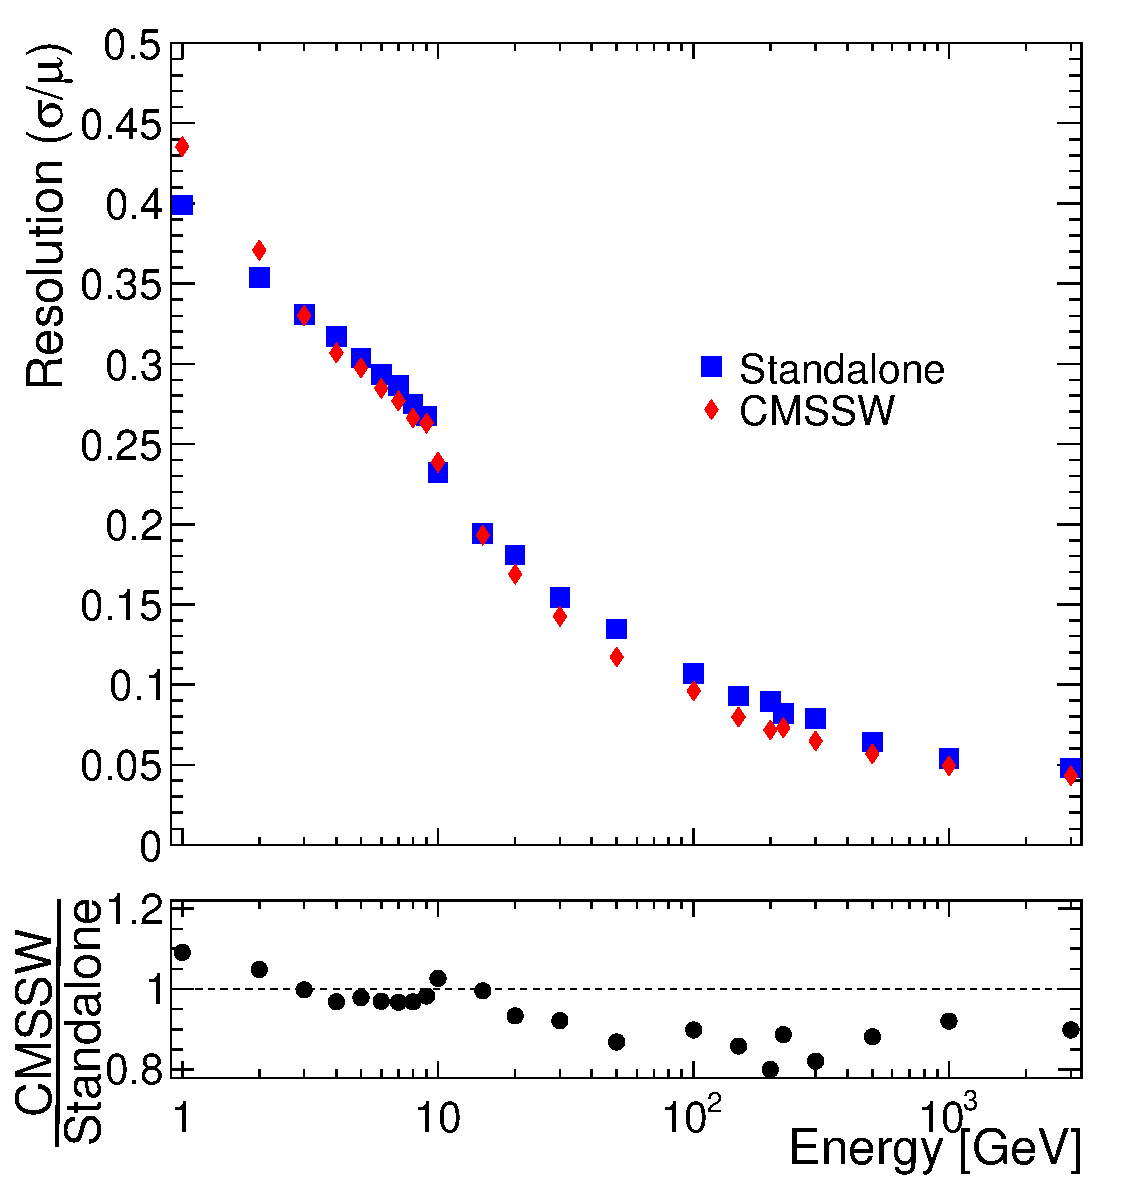
\includegraphics[width=0.49\textwidth]{figures/hcal_sigma_comp_tot.pdf}
\caption{Comparison between the standalone simulation and the CMSSW full simulation for pion energy response (left) and resolution (right).}
\label{fig:valplots}
\end{center}
\end{figure}

\subsection{Tests of Physics Effects on Pion Response and Resolution}
\label{sec:newdettests}

The pion response shown in Fig. \ref{fig:valplots} is highly nonlinear, especially at lower energies. The simplicity and flexibility of the standalone simulations makes it straightforward to test the various physics and geometrical effects identified in the preceding section. In order to test each effect individually, the simulation starts from the ``old default'' settings of the standalone simulation, before the validation against the CMSSW full simulation. The ``old default'' settings are: no preshower, minimal dead material (1.5\unit{mm}), and no Birks' Law in the ECAL or the zero layer. From here, each test setting is turned on by itself, without any of the others. Setting 5 is an additional test, removing Birks' Law from all of the HCAL scintillating layers. Changing the zero layer weight from 0.5 to 1.0 was also tested. The ``new default'' settings are those which were used to validate the standalone simulation; they consist of the ``old default'' settings with test settings 1, 2, 3, 4 applied in concert. For each test, the sampling factor $f_{\text{hcal}}$ was recalculated from 50\GeV pions simulated with the appropriate settings.

\begin{table}[hbtp]
\begin{center}
\caption{List of test settings}
\label{tab:testlist}
\begin{tabular}{l l}
0. & Old default: no preshower, no Birks' law in the ECAL or zero layer, \\
   & 1.5\unit{mm} of dead material \\
1. & 0 + inclusion of preshower \\
2. & 0 + Birks' Law in the ECAL \\
3. & 0 + dead material increased to 234\unit{mm} \\
4. & 0 + Birks' Law in the zero layer \\
5. & 0 + no Birks' Law in the HCAL \\
6. & New default: 0 + 1 + 2 + 3 + 4
\end{tabular}
\end{center}
\end{table}

Figure \ref{fig:testresp} shows the energy response from a Gaussian fit for 8\GeV and 50\GeV pions. The dead material between the ECAL and the HCAL has the largest effect on response, and Birks' Law in the HCAL scintillators also has a large effect. The preshower detector in front of the ECAL has a larger effect on the lower-energy pion response, as expected. Weighting the zero layer equal to the other layers increases the response and also improves the resolution for higher-energy pions when dead material is present, as shown in Fig. \ref{fig:testreso}. The presence of the preshower detector is the largest contribution to the resolution for lower-energy pions.

%figure: test response plots
\begin{figure}[hbtp]
\begin{center}
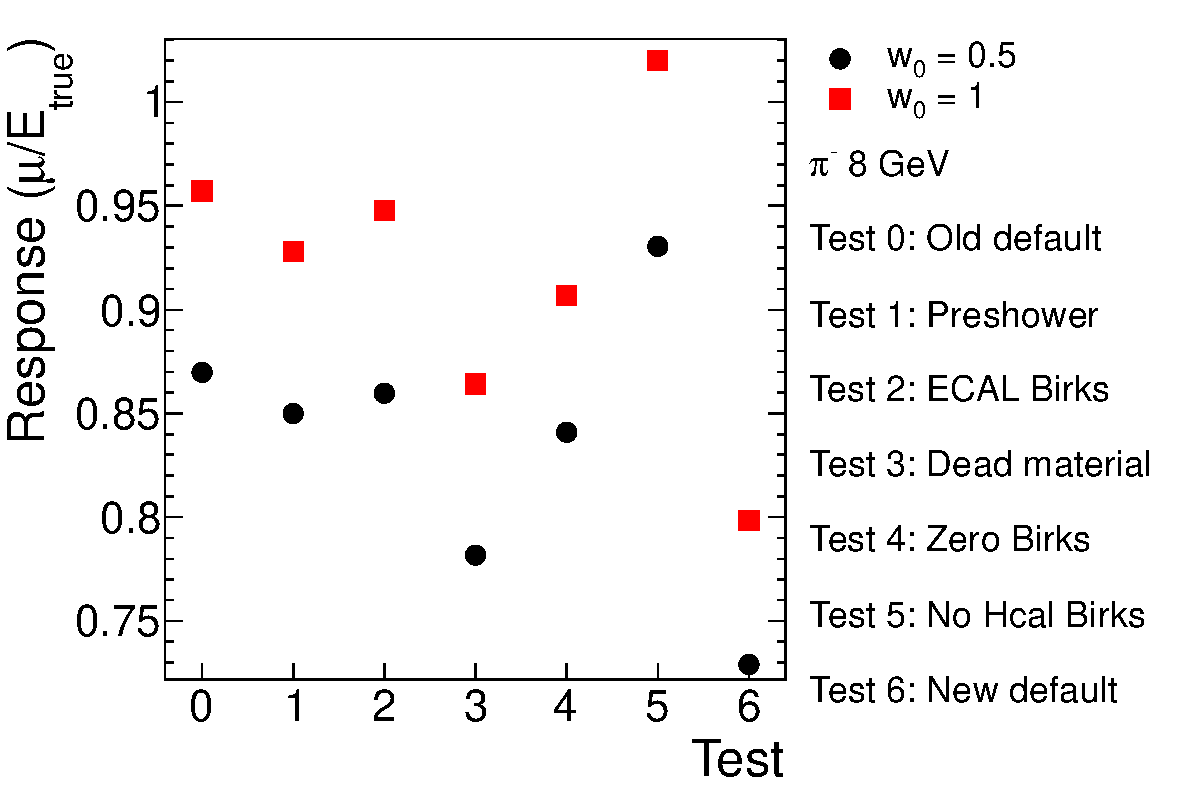
\includegraphics[width=0.49\textwidth]{figures/hcal_test_8gev_mu_tot.pdf}
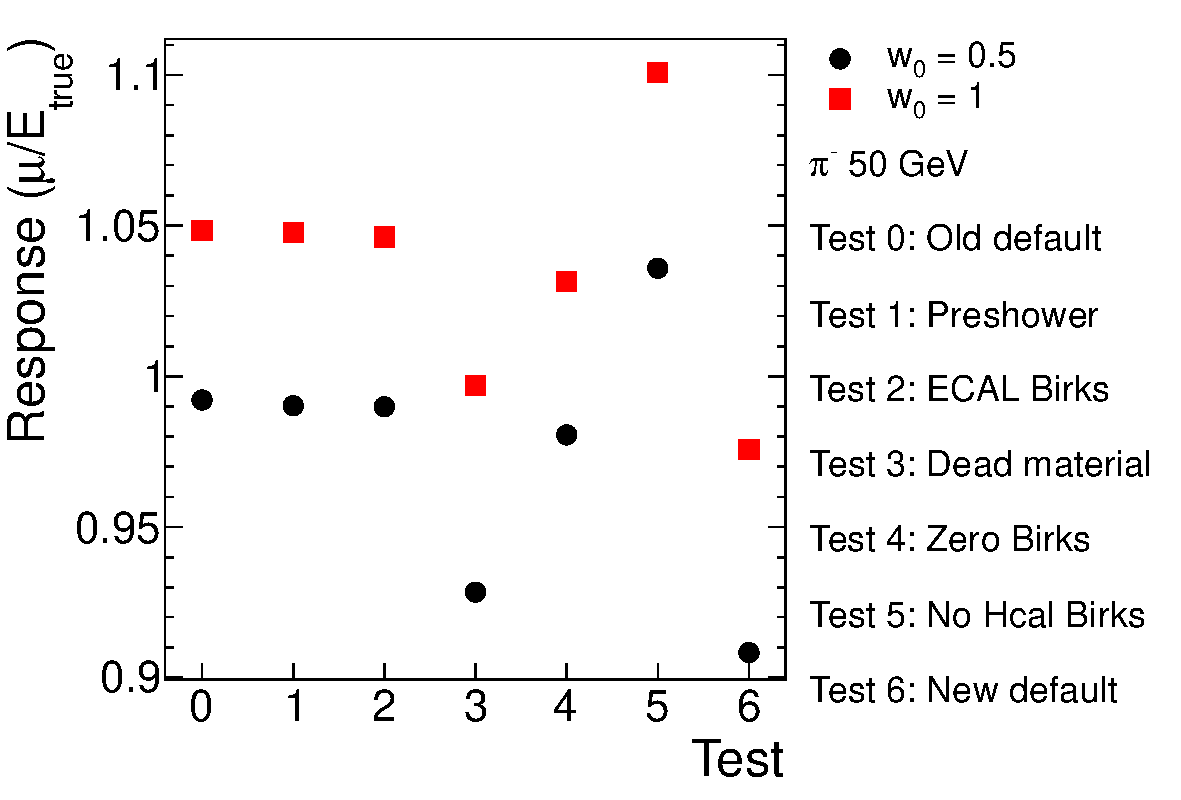
\includegraphics[width=0.49\textwidth]{figures/hcal_test_50gev_mu_tot.pdf}
\caption{Comparison of energy response for pions at 8\GeV (left) and 50\GeV (right), using test settings given in Table \ref{tab:testlist}.}
\label{fig:testresp}
\end{center}
\end{figure}

%figure: test resolution plots
\begin{figure}[hbtp]
\begin{center}
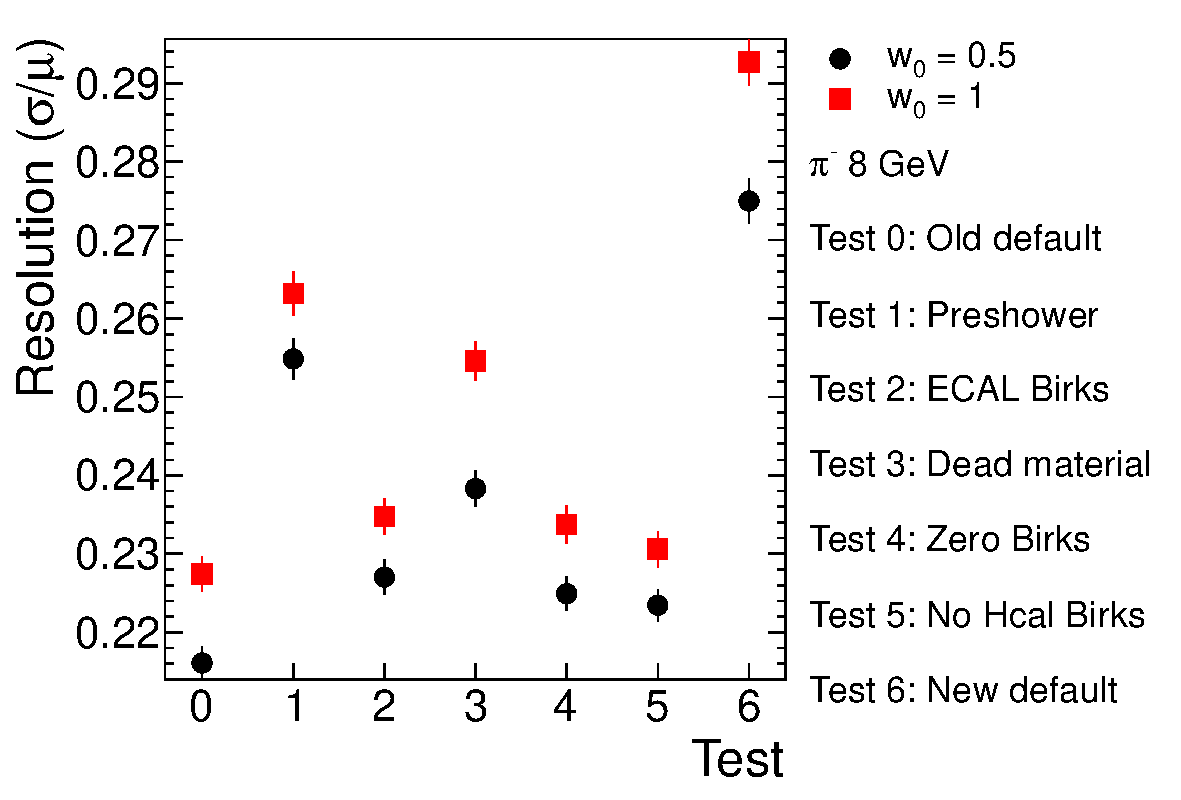
\includegraphics[width=0.49\textwidth]{figures/hcal_test_8gev_sigma_tot.pdf}
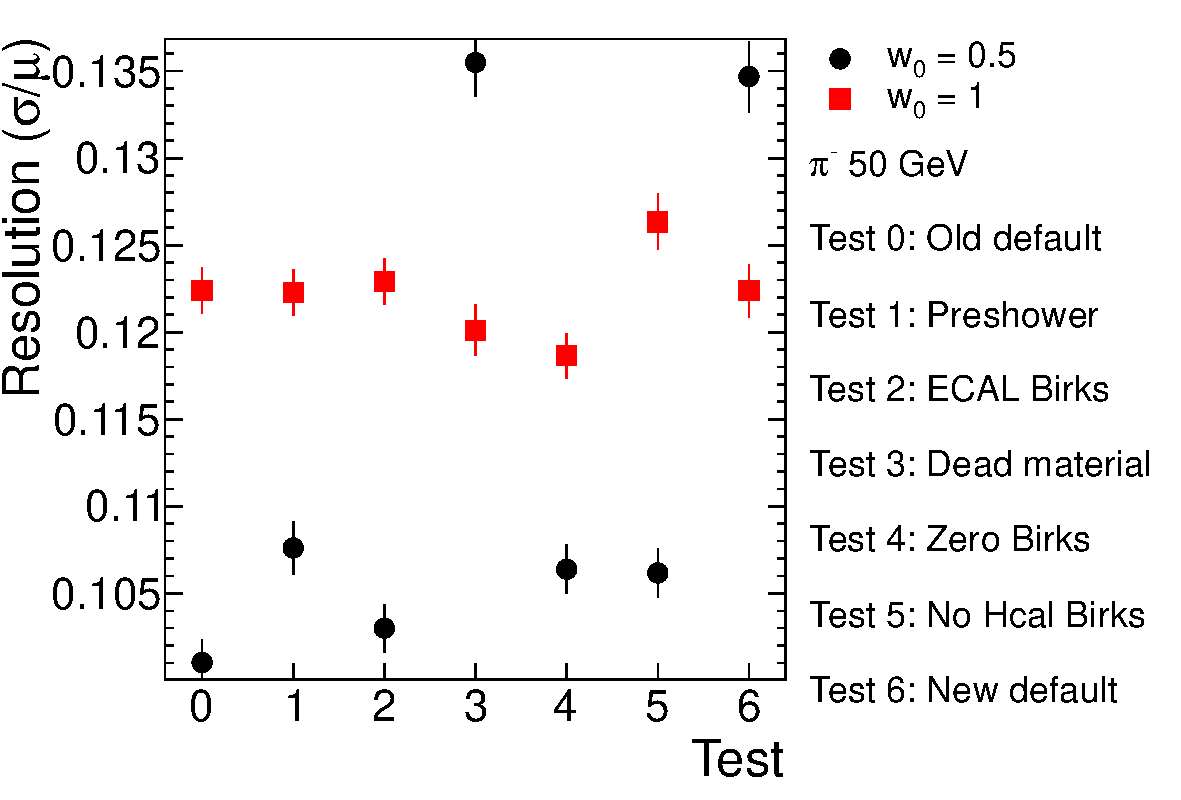
\includegraphics[width=0.49\textwidth]{figures/hcal_test_50gev_sigma_tot.pdf}
\caption{Comparison of energy resolution for pions at 8\GeV (left) and 50\GeV (right), using test settings given in Table \ref{tab:testlist}.}
\label{fig:testreso}
\end{center}
\end{figure}

\subsection{HE Rebuild/Extension + Shashlik ECAL Physics Studies}

%needs to be rewritten from version in AN-12-447, todo

\section{Hadronic Fast Simulation}

The CMS hadronic fast simulation is based on the mean shower parameterization from GFLASH \cite{gflash}, containing one term for the hadronic component and another term for the $\pi^{0}$ (electromagnetic) component. Various random fluctuations for the longitudinal and transverse development and the energy deposition of the shower are included in the simulation. However, the GFLASH parameterization for hadronic showers was only developed for single homogeneous calorimeters. The CMS HCAL is a sampling calorimeter with a non-compensating homogeneous crystal ECAL and dead material in front of it. The final energy measured by this combined calorimeter system for a given event is the product of not just shower fluctuations, but also sampling fluctuations, non-linearity, and geometric effects. To include these other effects, the energy deposits from the fast simulation must be multiplied by a random factor generated according to hadronic energy distributions from the full simulation (``smeared'').

%will be heavily expanded with plots, etc...
\subsection{Retuning of Hadronic Response}

At first, Gaussian distributions were used for the hadronic energy response smearing. The parameters for the Gaussian distributions were taken from the means and standard deviations of energy distributions for single pion samples from the full simulation. The energy distributions were constructed by collecting reconstructed calorimeter hits in a cone of $\Delta R < 0.5$, divided into bins of $\Delta \eta = 0.1$ based on the incident pion direction. These samples were simulated at different energies and the Gaussian parameters were linearly interpolated for intermediate energies. Additional $\eta$- and energy-dependent factors were derived to improve agreement with the full simulation, accounting for any remaining differences between the simulations in an ad-hoc, rather than physical, way.

The fast simulation of the calorimeters originally used a custom reconstruction process. However, to make the simulations easier to maintain and upgrade, the fast simulation was changed to use the full digitization and reconstruction, which are described in Ch. \ref{ch:digireco}, without significant loss in speed. This change invalidated the ad-hoc correction factors described above, which were derived from the custom reconstruction process for the response smearing based on reconstructed hits. A new, more precise tuning, based on simulated hits, would ideally work well enough to omit any ad-hoc correction factors.

A simple Gaussian distribution does not capture potential large tails in the pion energy distributions. To account for the behavior of both the low- and high-energy tails, a double-sided Crystal Ball function is used. This function has a Gaussian core with two power-law tails. The Crystal Ball function is continuous, and despite being defined in a piecewise manner, so is its first derivative. In order to generate random numbers distributed according to a double-sided Crystal Ball function, inversion sampling is used. The cumulative distribution function of the double-sided Crystal Ball function is invertible, enabling the random generation to be computed analytically, up to the calculation of the error function erf.

To describe this method, first the probability distribution function (PDF) $f(x)$ and the cumulative distribution function (CDF) $F(x)$ must be defined in general:
\begin{align}
\int_{-\infty}^{\infty} f(x)dx &= 1 \\
F(x) &= \int_{-\infty}^{x} f(x^{\prime})dx^{\prime} \label{eq:generalCDF} \\
y \equiv F(x) &\rightarrow F^{-1}(y) = x \label{eq:inverseCDF}
\end{align}
Equation \eqref{eq:inverseCDF} shows the basis of inversion sampling: the inverted CDF $F^{-1}(y)$ produces a random number distributed according to the PDF $f(x)$.

The double-sided Crystal Ball function has six parameters as noted below, with a few additional definitions and conditions:
\begin{align}
\vec{p} &= (\mu,\sigma,a_{L},n_{L},a_{R},n_{R}) \\
d_{L} &= n_{L}/a_{L} \\
d_{R} &= n_{R}/a_{R} \\
n_{L}, n_{R} &> 1\\
a_{L}, a_{R} &> 0
\end{align}
Here, $\mu$ is the mean of the Gaussian core, $\sigma$ is the width of the Gaussian core, $a_{L}$ is the starting location of the left tail, $n_{L}$ is the steepness of the left tail, and $a{R}$ and $n_{R}$ act similarly for the left tail. The parameter combinations $d_{L}$ and $d_{R}$ appear frequently in the definition of the Crystal Ball function, so it is useful to define them. The conditions on $n_{L}$ and $n_{R}$ ensure that the Crystal Ball function has a finite integral and can be used as a PDF, while the conditions on $a_{L}$ and $a_{R}$ ensure that the function is continuous. The PDF of the Crystal Ball, using these parameters, is given in Eq. \eqref{eq:cballPDF}, with the normalization given in Eq. \eqref{eq:cballnorm}.

\begin{equation}
f(x;\vec{p}) = N \cdot \begin{cases}
\text{exp}\left(-\frac{a_{L}^{2}}{2}\right) \cdot \left[\frac{1}{d_{L}}\left(d_{L} - a_{L} - \frac{x-\mu}{\sigma}\right)\right]^{-n_{L}} & \text{for $\frac{x-\mu}{\sigma} \leq -a_{L}$} \\
\\
\text{exp}\left(-\frac{1}{2}\left(\frac{x-\mu}{\sigma}\right)^2\right) & \text{for $-a_{L} < \frac{x-\mu}{\sigma} < a_{R}$} \\
\\
\text{exp}\left(-\frac{a_{R}^{2}}{2}\right) \cdot \left[\frac{1}{d_{R}}\left(d_{R} - a_{R} + \frac{x-\mu}{\sigma}\right)\right]^{-n_{R}} & \text{for $\frac{x-\mu}{\sigma} \geq a_{R}$}
\end{cases}
\label{eq:cballPDF}
\end{equation}

\begin{equation}
N = \frac{1}{\sigma\left[\frac{d_{L}}{n_{L}-1} \cdot \text{exp}\left(-\frac{a_{L}^{2}}{2}\right) + \sqrt{\frac{\pi}{2}}\left(\text{erf}\left(\frac{a_{L}}{\sqrt{2}}\right)+\text{erf}\left(\frac{a_{R}}{\sqrt{2}}\right)\right) + \frac{d_{R}}{n_{R}-1} \cdot \text{exp}\left(-\frac{a_{R}^{2}}{2}\right)  \right]}
\label{eq:cballnorm}
\end{equation}

The PDF can be integrated according to Eq. \eqref{eq:generalCDF} to produce the CDF in Eq. \eqref{eq:cballCDF}. The same CDF is shown in shortened form in Eq. \eqref{eq:cballCDF2}, with some abbreviations defined to make the inverse CDF in Eq. \eqref{eq:cballCDFinv} more readable.

\begin{align}
F(x;\vec{p}) &= \sigma N \cdot \begin{cases}
\frac{d_{L}}{n_{L}-1}\text{exp}\left(-\frac{a_{L}^2}{2}\right) \left[\frac{1}{d_{L}}\left(d_{L}-a_{L}-\frac{x-\mu}{\sigma}\right)\right]^{-n_{L}+1} & \text{for $\frac{x-\mu}{\sigma} \leq -a_{L}$} \\
\\
\frac{d_{L}}{n_{L}-1}\text{exp}\left(-\frac{a_{L}^2}{2}\right) + \sqrt{\frac{\pi}{2}}\text{erf}\left(\frac{a_{L}}{\sqrt{2}}\right) + \sqrt{\frac{\pi}{2}}\text{erf}\left(\frac{x-\mu}{\sigma \sqrt{2}}\right) & \text{for $-a_{L} < \frac{x-\mu}{\sigma} < a_{R}$} \\
\\
\frac{d_{L}}{n_{L}-1}\text{exp}\left(-\frac{a_{L}^2}{2}\right) + \sqrt{\frac{\pi}{2}}\text{erf}\left(\frac{a_{L}}{\sqrt{2}}\right)\\
 + \sqrt{\frac{\pi}{2}}\text{erf}\left(\frac{a_{R}}{\sqrt{2}}\right) + \frac{d_{R}}{n_{R}-1}\text{exp}\left(-\frac{a_{R}^2}{2}\right) \\
 + \frac{d_{R}}{1-n_{R}}\text{exp}\left(-\frac{a_{R}^2}{2}\right) \left[\frac{1}{d_{R}}\left(d_{R}-a_{R}+\frac{x-\mu}{\sigma}\right)\right]^{-n_{R}+1} & \text{for $\frac{x-\mu}{\sigma} \geq a_{R}$}
\end{cases}\label{eq:cballCDF}\\
 &= \sigma N \cdot \begin{cases}
B_{L} \left[\frac{1}{d_{L}}\left(d_{L}-a_{L}-\frac{x-\mu}{\sigma}\right)\right]^{-n_{L}+1} & \text{for $\frac{x-\mu}{\sigma} \leq -a_{L}$} \\
\\
A_{L} + C_{L} + \sqrt{\frac{\pi}{2}}\left(1-\text{erfc}\left(\frac{x-\mu}{\sigma \sqrt{2}}\right)\right) & \text{for $-a_{L} < \frac{x-\mu}{\sigma} < a_{R}$} \\
\\
A_{L} + C_{L} + C_{R} + A_{R} \\
 + B_{R} \left[\frac{1}{d_{R}}\left(d_{R}-a_{R}+\frac{x-\mu}{\sigma}\right)\right]^{-n_{R}+1} & \text{for $\frac{x-\mu}{\sigma} \geq a_{R}$} \\
\end{cases}\label{eq:cballCDF2}
\end{align}

\begin{equation}
x = \begin{cases}
\mu + \sigma \left(-d_{L}\left[\frac{y}{\sigma N}/B_{L}\right]^{\frac{1}{-n_{L}+1}}-a_{L}+d_{L} \right) & \text{for $y < \sigma N A_{L}$} \\
\\
\mu + \sigma \sqrt{2} \text{erfc}^{-1}\left[1-\sqrt{\frac{2}{\pi}}\left(\frac{y}{\sigma N}-A_{L}-C_{L}\right)\right] & \text{for $\sigma N A_{L} \leq y \leq \sigma N (A_{L} + C_{L} + C_{R})$} \\
\\
\mu + \sigma \left(d_{R}\left[\frac{\frac{y}{\sigma N} - A_{L} - C_{L} - C_{R} - A_{R}}{B_{R}}\right]^{\frac{1}{-n_{R}+1}}+a_{R}-d_{R}\right) & \text{for $y > \sigma N (A_{L} + C_{L} + C_{R})$}
\end{cases}
\label{eq:cballCDFinv}
\end{equation}

This inverse CDF is used for the inversion sampling procedure. A uniform random number $y$ is generated and used as the input to Eq. \eqref{eq:cballCDFinv}, producing $x$ which is distributed according to the double-sided Crystal Ball function.

Charged pion events are used to determine the double-sided Crystal Ball parameter values for the hadronic response smearing. For each of several energy values (1, 2, 3, 5, 9, 11, 15, 20, 30, 50, 100, 150, 225, 300, 1000, 3000\GeV), a sample of 500,000 pion events was generated, uniformly distributed in $|\eta|<5.0$, and simulated using the full simulation. Vertex smearing and the magnetic field were disabled, so the direction of the incident pion would directly predict the location of energy deposits in the calorimeter. Energy from ECAL and HCAL simulated hits was collected in a cone of $\Delta R < 0.5$. The HCAL energy was calibrated by multiplying by the $\eta$-dependent sampling factors determined in the full simulation.

For each energy, the sample was divided into bins of $\Delta \eta = 0.1$. Each resulting energy distribution was fit to a double-sided Crystal Ball function. For these fits, the default energy range was $[0.1E,2E]$ where $E$ is the true energy, and the parameter limits were: $\mu, \sigma > 0$; $0 \leq a_{L}, a_{R} \leq 10$; $1.01 \leq n_{L}, n_{R} \leq 200$. Technically, the Crystal Ball function approaches a Gaussian function when $a \rightarrow \infty$. However, because the $a$ parameters are in units of $\sigma$, $a = 10$ is effectively infinite in practice. The chance of a $10\sigma$ event occurring randomly, if the events are normally distributed, is approximately 1 in 66 sextillion. The energy range and parameter values were slightly altered in some cases when the $\chi^{2}$ value of the fit indicated that the fitting algorithm was trapped in a bad local minimum. Examples of the energy distributions and double-sided Crystal Ball fits are shown in Fig. \ref{fig:cballD-fits}.

%figure: cballD fit examples
\begin{figure}[hbtp]
\begin{center}
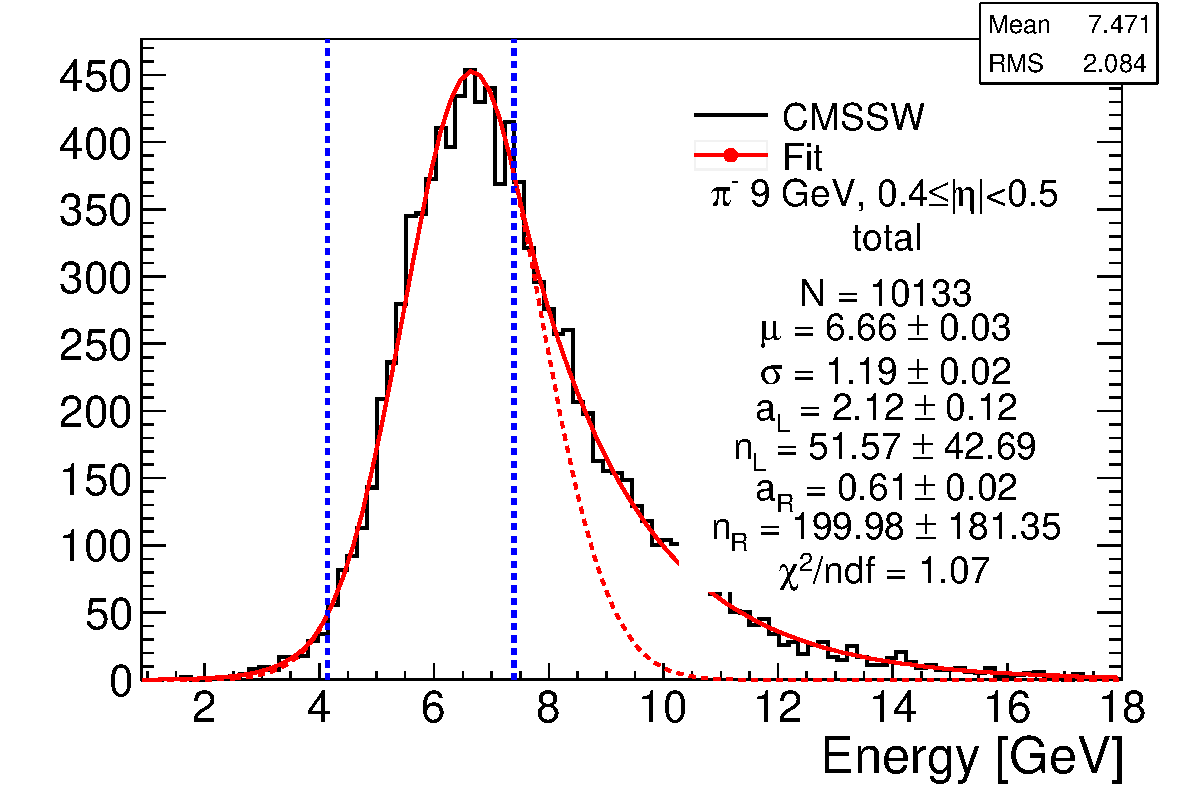
\includegraphics[width=0.49\textwidth]{figures/pion_response_tot_cballD_9gev_ieta5.pdf}
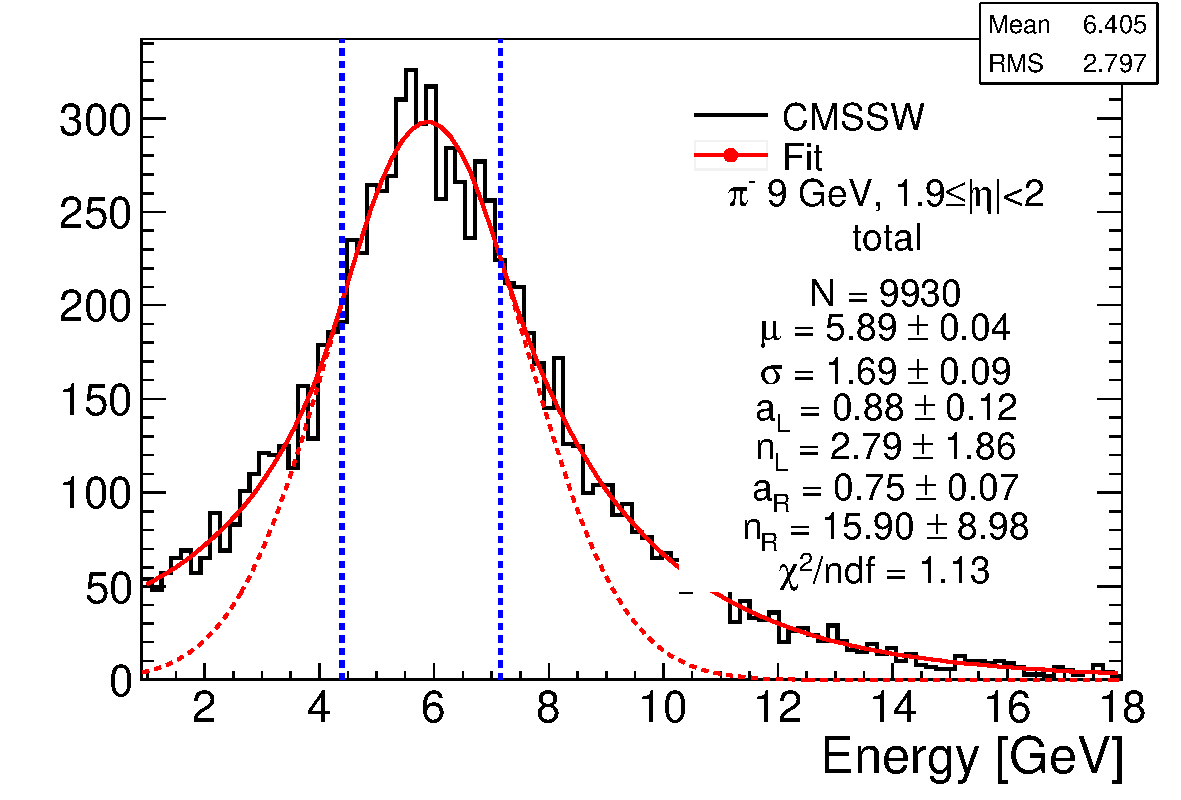
\includegraphics[width=0.49\textwidth]{figures/pion_response_tot_cballD_9gev_ieta20.pdf}
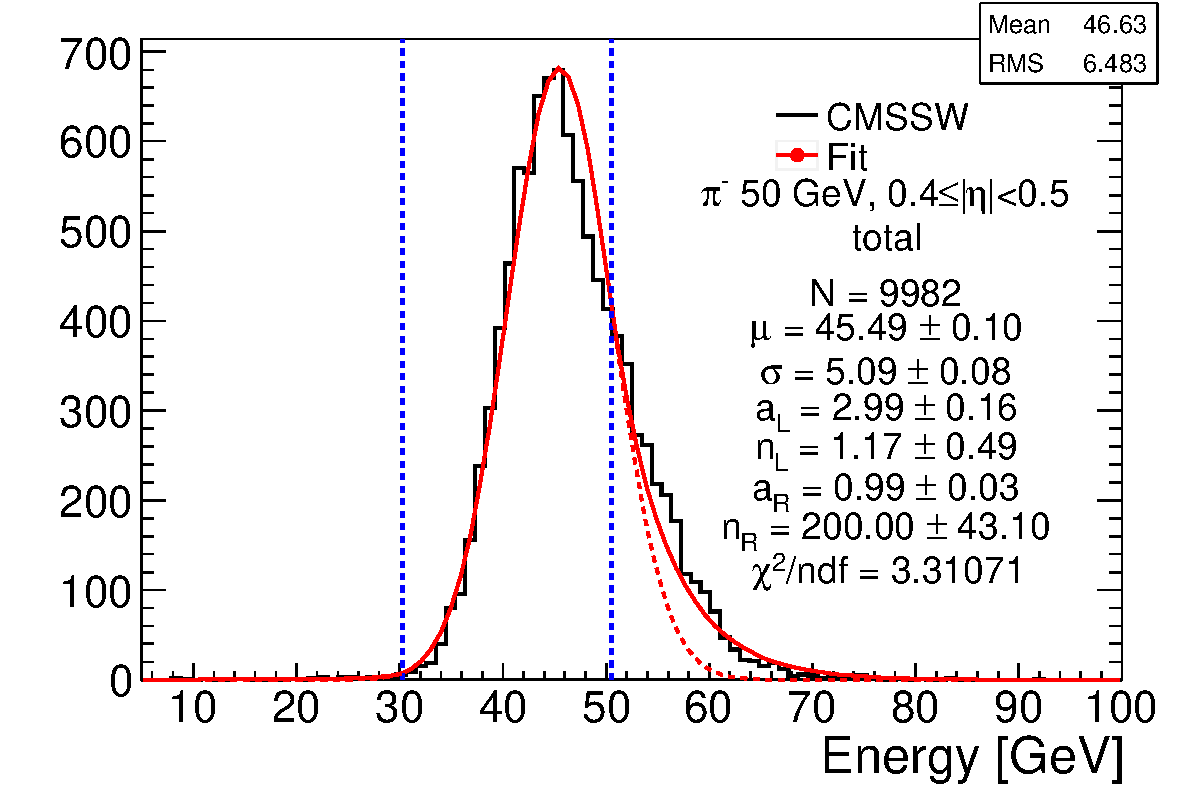
\includegraphics[width=0.49\textwidth]{figures/pion_response_tot_cballD_50gev_ieta5.pdf}
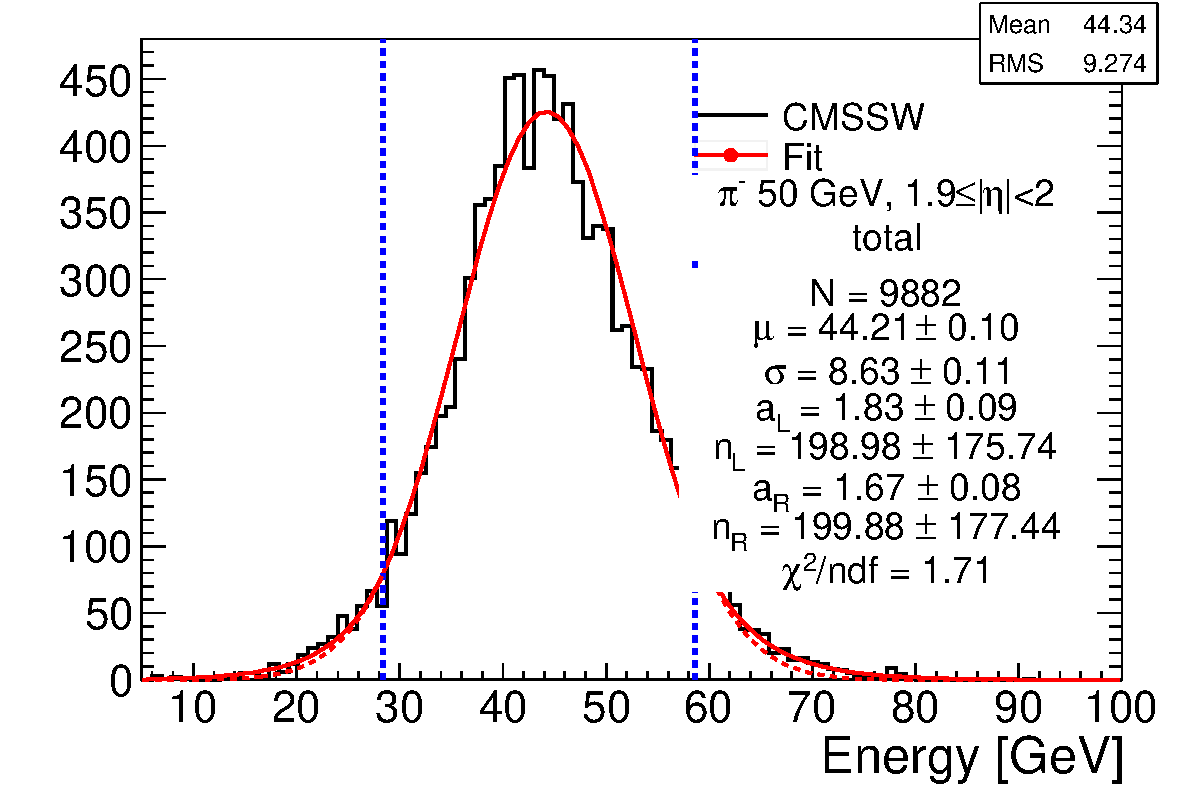
\includegraphics[width=0.49\textwidth]{figures/pion_response_tot_cballD_50gev_ieta20.pdf}
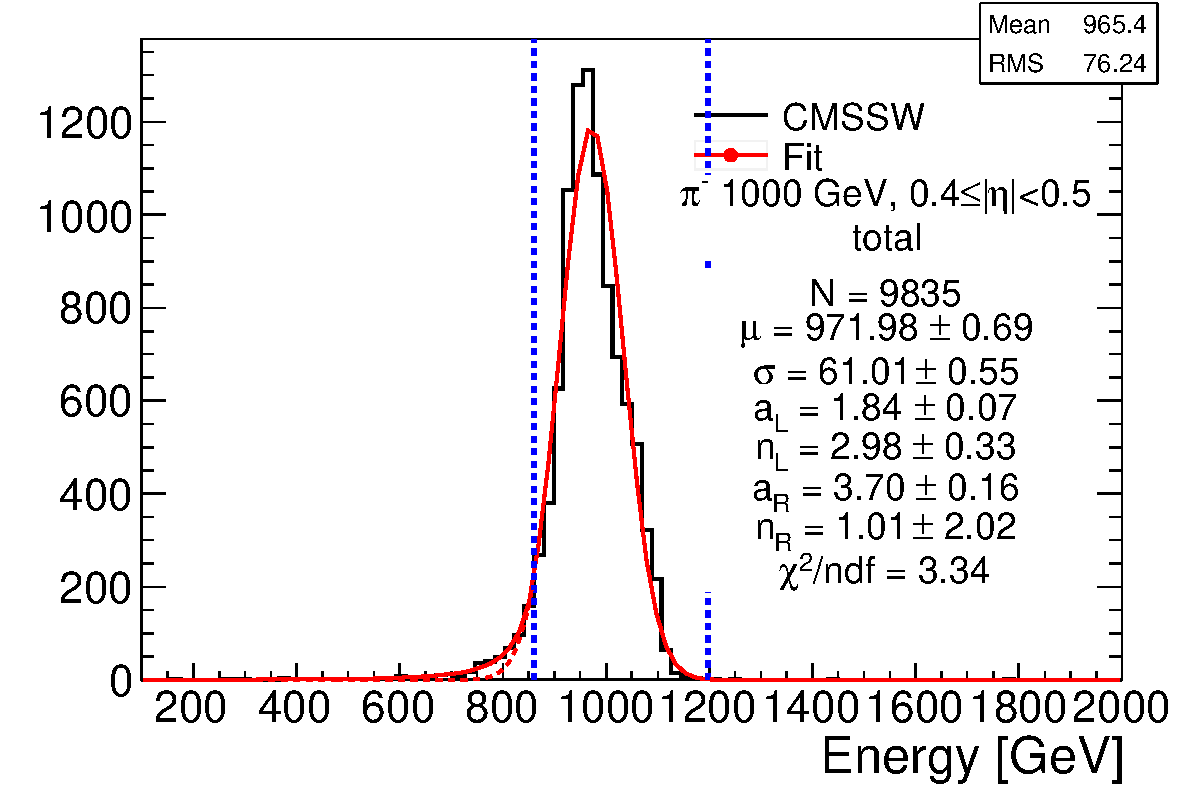
\includegraphics[width=0.49\textwidth]{figures/pion_response_tot_cballD_1000gev_ieta5.pdf}
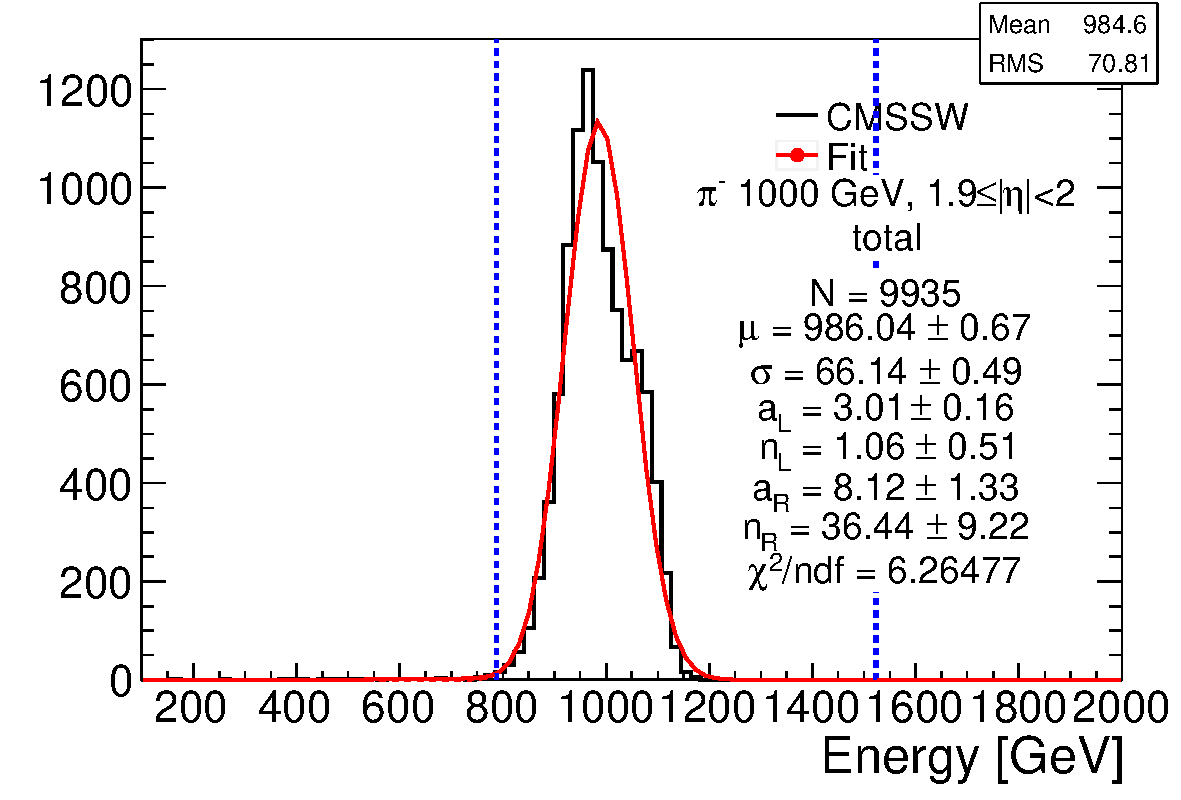
\includegraphics[width=0.49\textwidth]{figures/pion_response_tot_cballD_1000gev_ieta20.pdf}
\caption{Examples of double-sided Crystal Ball fits to simulated pion energy distributions. Low (top), medium (middle), and high (bottom) energies are displayed for $\eta$ ranges in the barrel (left) and endcap (right). The blue dotted lines show the locations of the transition from the Gaussian core to the power-law tails, and the red dotted lines show a continuation of the Gaussian core for comparison to the power-law tails.}
\label{fig:cballD-fits}
\end{center}
\end{figure}

For the response smearing, the parameter values resulting from the fits are linearly interpolated for intermediate energies that were not explicitly simulated. This linear interpolation routine includes safety checks when used for extrapolation beyond the simulated energy range, to prevent any unphysical parameter values. The parameter values, including the linear interpolation, are shown in Fig. \ref{fig:cballD-params}. The values of the $\mu$ and $\sigma$ parameters are shown in the more familiar forms of fractional response $\mu/E_{\text{true}}$ and fractional resolution $\sigma/\mu$. Some trends can be observed in these parameter values. The expected nonlinearity in fractional response versus energy is present, and the boundaries between different subdetectors are apparent. The expected decrease in fractional resolution as energy increases is also present. The $a_{R}$ and $n_{R}$ plots show the disappearance of the right-side tail with increasing energy in the barrel and endcap. The $a_{R}$ values increase, indicating that the tail starts further from the Gaussian peak and contains fewer events, and the $n_{R}$ values also increase, indicating that the tail becomes steeper. The reduced $\chi^{2}$ values for each fit are shown in Fig. \ref{fig:cballD-chi2}.

%figure: cballD parameter values
\begin{figure}[hbtp]
\begin{center}
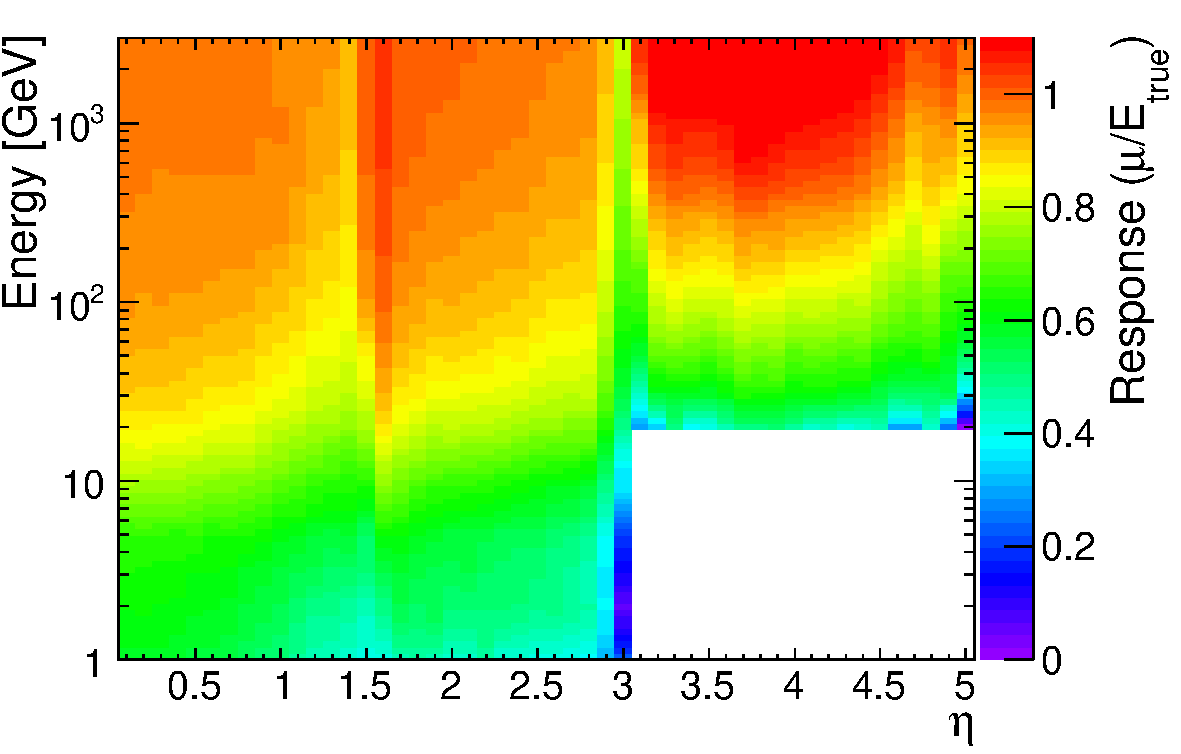
\includegraphics[width=0.49\textwidth]{figures/mu_tot_interp.pdf}
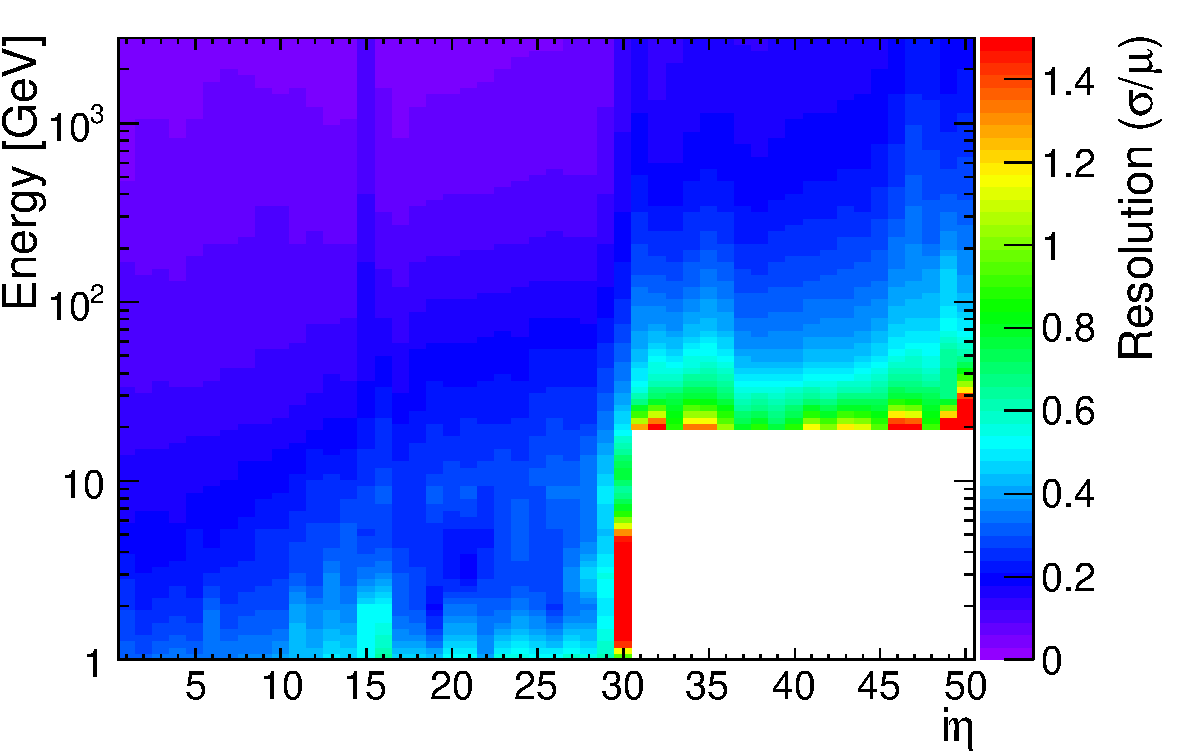
\includegraphics[width=0.49\textwidth]{figures/sigma_tot_interp.pdf}
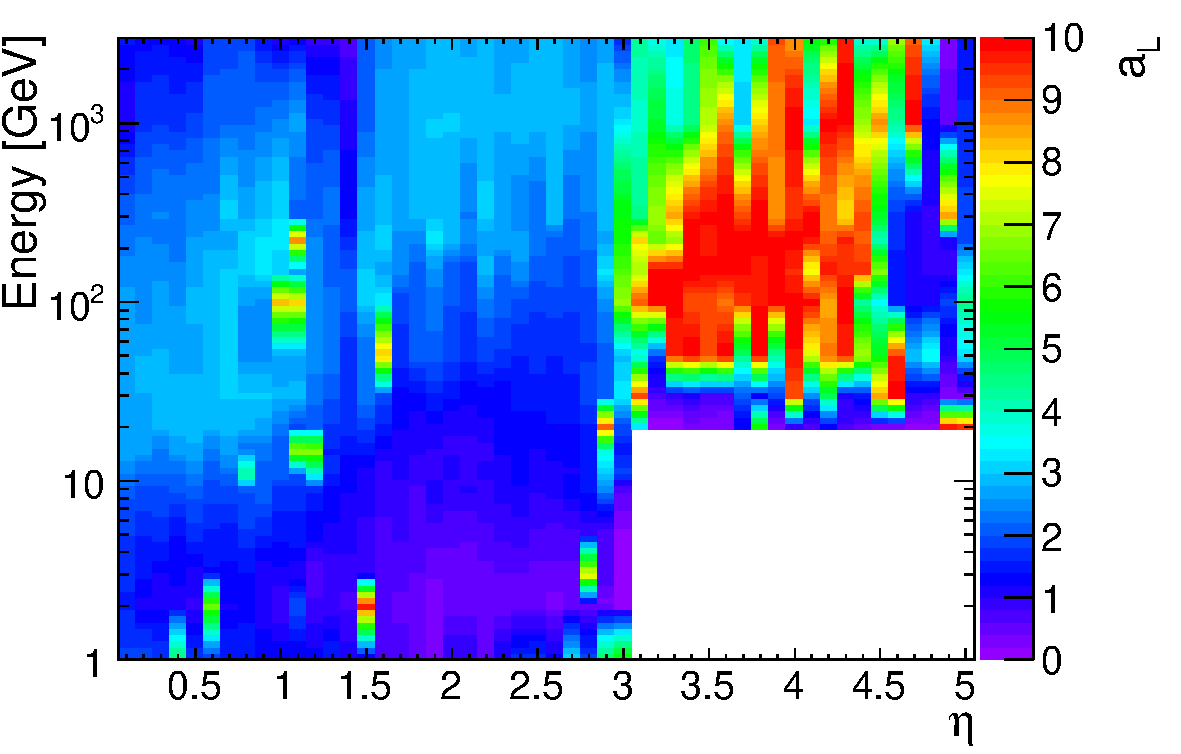
\includegraphics[width=0.49\textwidth]{figures/aL_tot_interp.pdf}
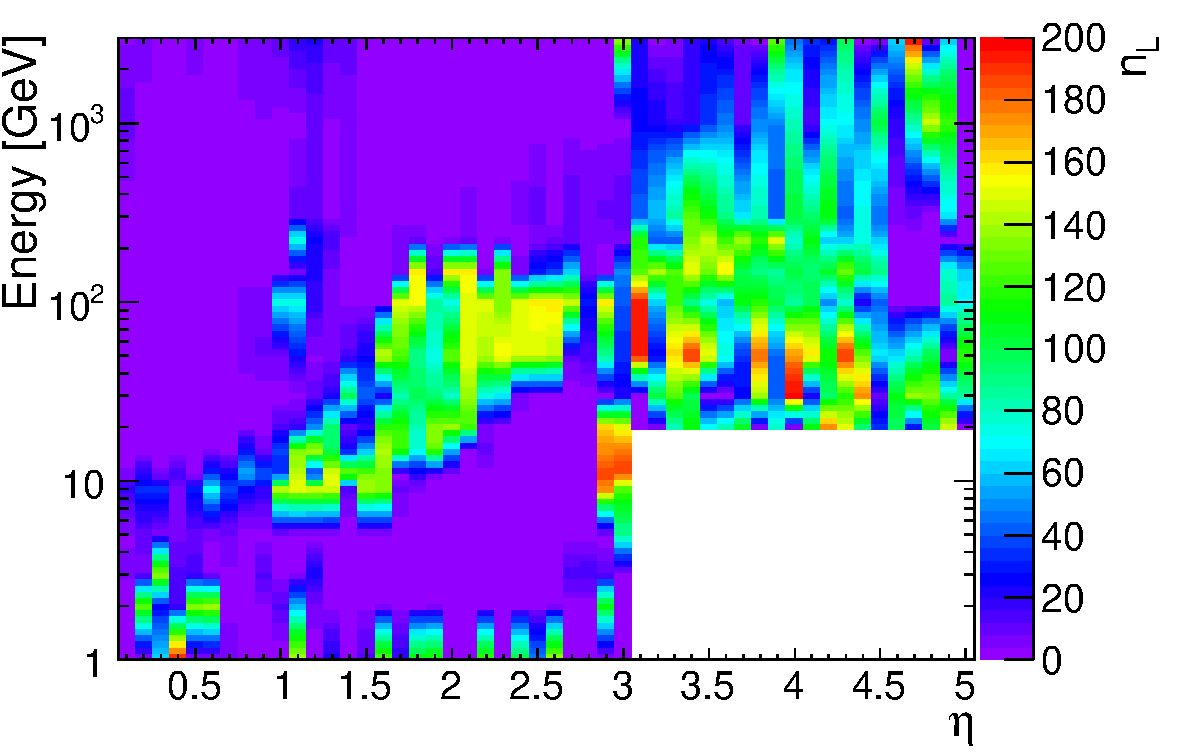
\includegraphics[width=0.49\textwidth]{figures/nL_tot_interp.pdf}
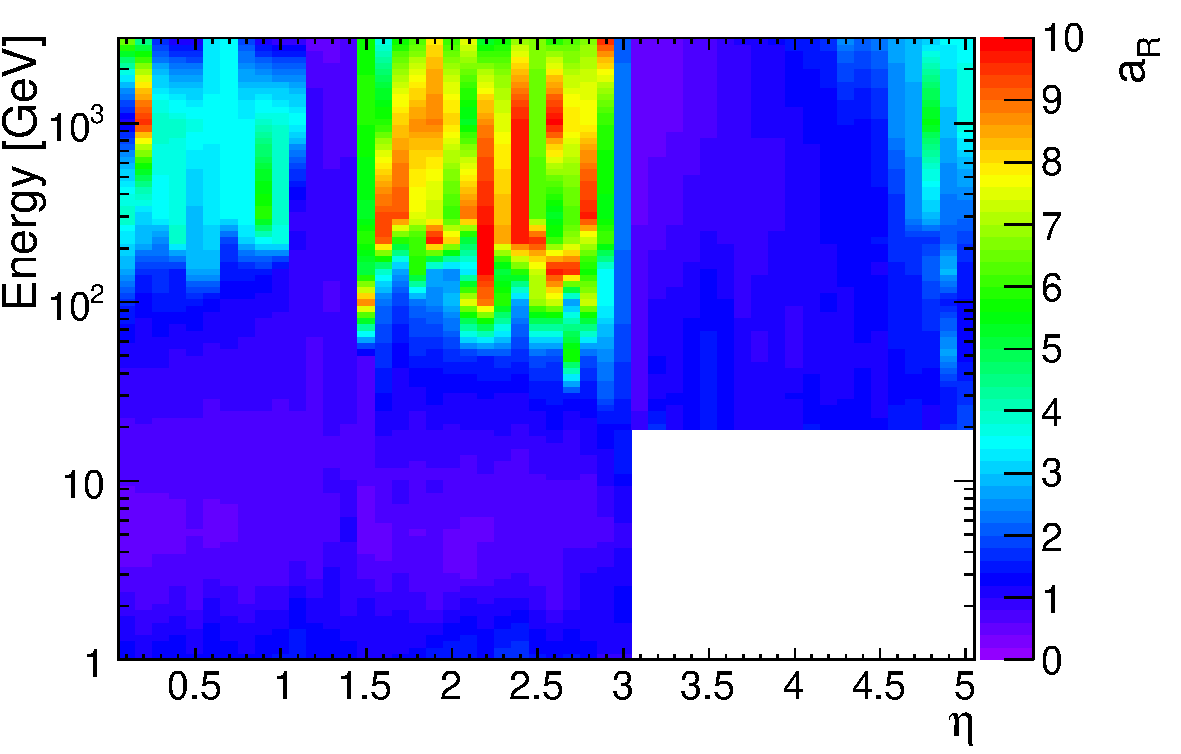
\includegraphics[width=0.49\textwidth]{figures/aR_tot_interp.pdf}
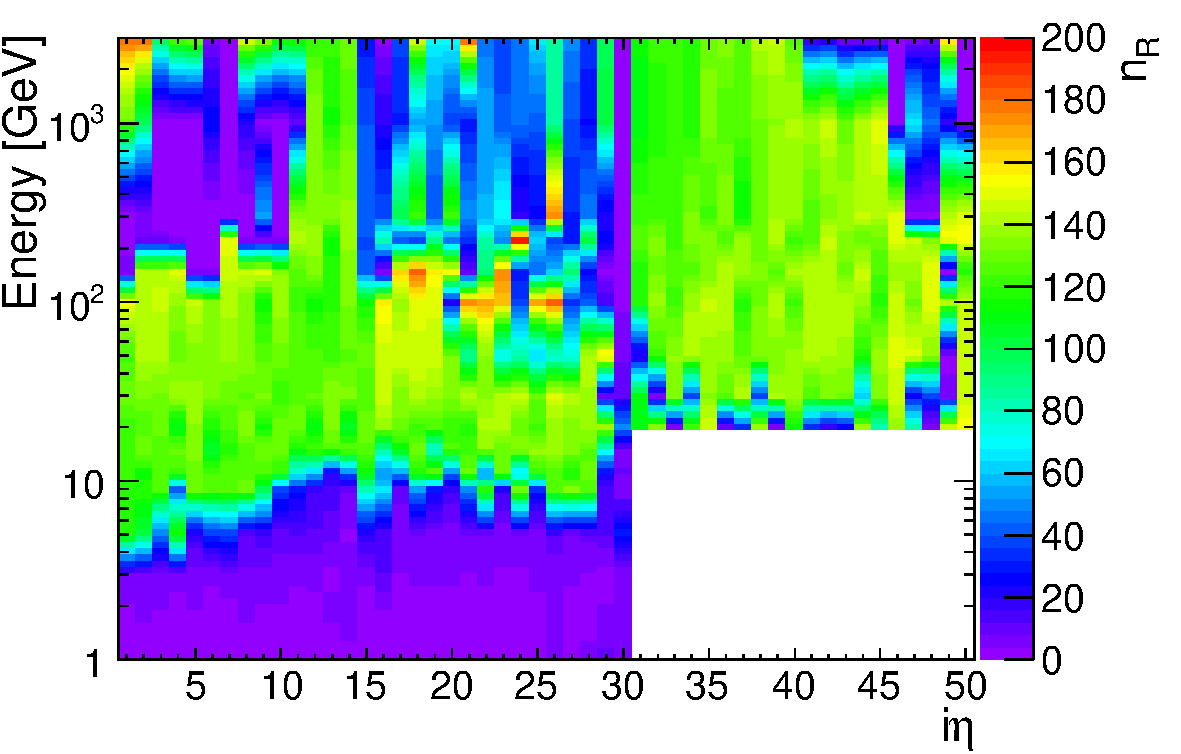
\includegraphics[width=0.49\textwidth]{figures/nR_tot_interp.pdf}
\caption{Parameter values for the double-sided Crystal Ball fits, with linear interpolation for intermediate energy values: fractional response $\mu/E_{\text{true}}$ (top left), fractional resolution $\sigma/\mu$ (top right), $a_{L}$ (middle left), $n_{L}$ (middle right), $a_{R}$ (bottom left), $n_{R}$ (bottom right).}
\label{fig:cballD-params}
\end{center}
\end{figure}

\begin{figure}[hbtp]
  \begin{center}
    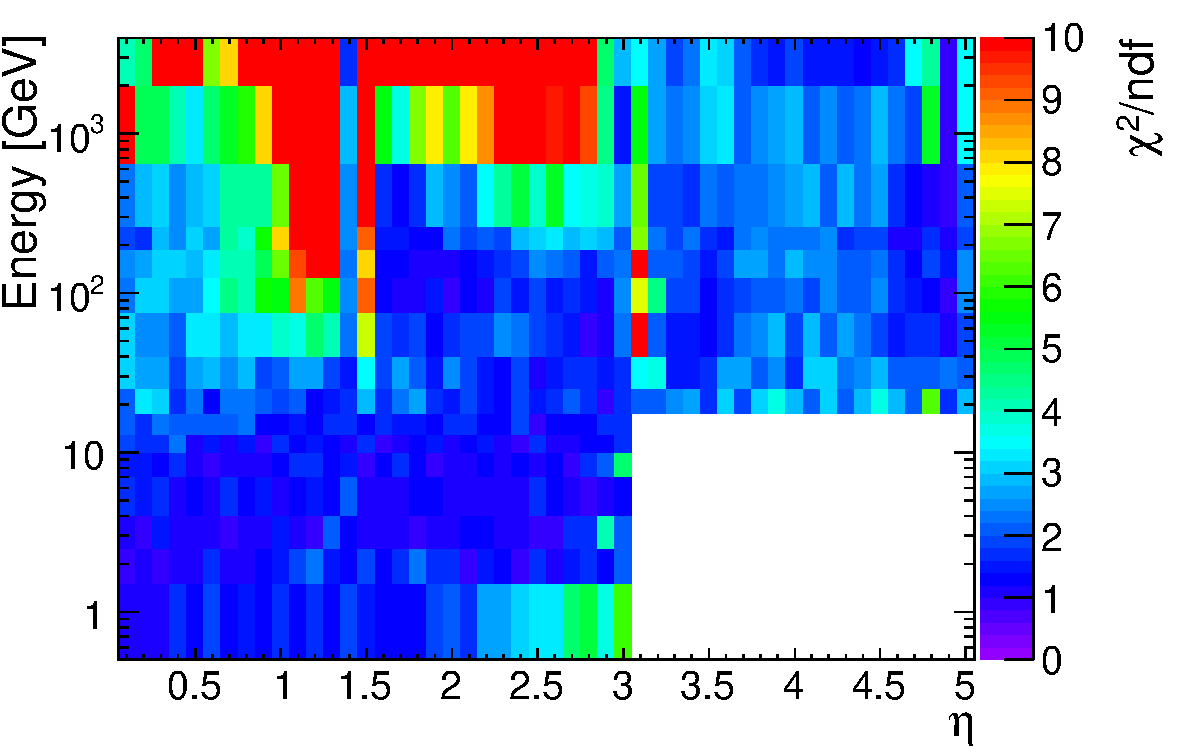
\includegraphics[width=0.98\textwidth]{figures/chi2_tot.pdf}
    \caption{Reduced $\chi^{2}$ values for each double-sided Crystal Ball fit.}
    \label{fig:cballD-chi2}
  \end{center}
\end{figure}

The low-energy region in the HF is excluded from Figs. \ref{fig:cballD-params} and \ref{fig:cballD-chi2}. The HF detects particles using Cherenkov light rather than scintillation light, so the yield of photoelectrons is much lower, typically 1 photoelectron per 4\GeV. Therefore, the energy distribution in the HF is Poissonian rather than Gaussian for low energy particles, so the double-sided Crystal Ball fit is not appropriate. An alternate approach is used in this region. The overall photoelectron distribution is fit with a Poissonian function, and a second Poissonian function is used to model the spread of values between integer numbers of photoelectrons. Examples of these fits are shown in Fig. \ref{fig:poissonHF-fits}. As with the Crystal Ball fits, the parameter values are interpolated when calculating response smearing factors for intermediate energy values. For energies below 5\GeV, the 5\GeV parameter values are used.

%figure: HF poisson fits from Reza
\begin{figure}[hbtp]
\begin{center}
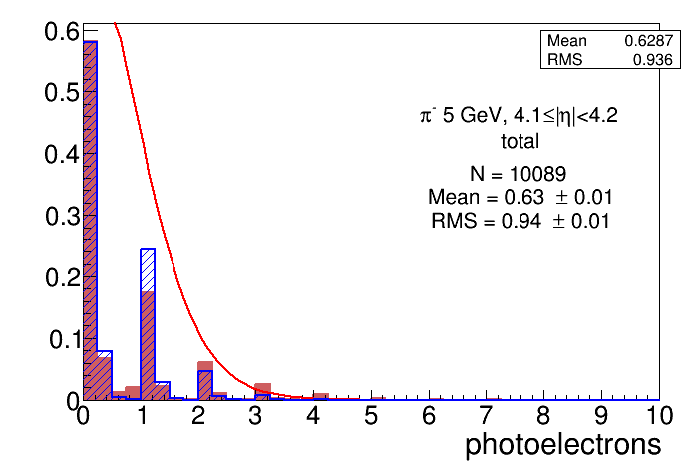
\includegraphics[width=0.49\textwidth]{figures/finaltaskreport_Page_5_Image_0004.png}
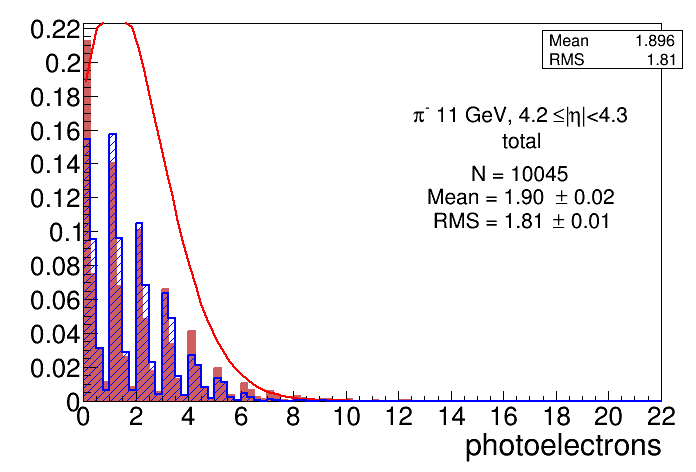
\includegraphics[width=0.49\textwidth]{figures/finaltaskreport_Page_5_Image_0005.png}
\caption{Poisson fits for low-energy photoelectron distributions in the HF \cite{Reza:HF}. The red histogram is the distribution, the red curve is the overall Poisson fit, and the blue hatched histogram is the result of randomly generated points using the Poisson fits. Plots are shown for 5\GeV (left) and 11\GeV (right) charged pion samples with $\eta$ ranges in the HF.}
\label{fig:poissonHF-fits}
\end{center}
\end{figure}

For higher energy particles in the HF, the distributions approach a Gaussian shape with possible large tails, so the double-sided Crystal Ball fit is used for these cases. Examples of the energy distributions and fits for the HF are shown in Fig. \ref{fig:cballD-fits-HF}.

%figure: cballD fit examples for HF
\begin{figure}[hbtp]
\begin{center}
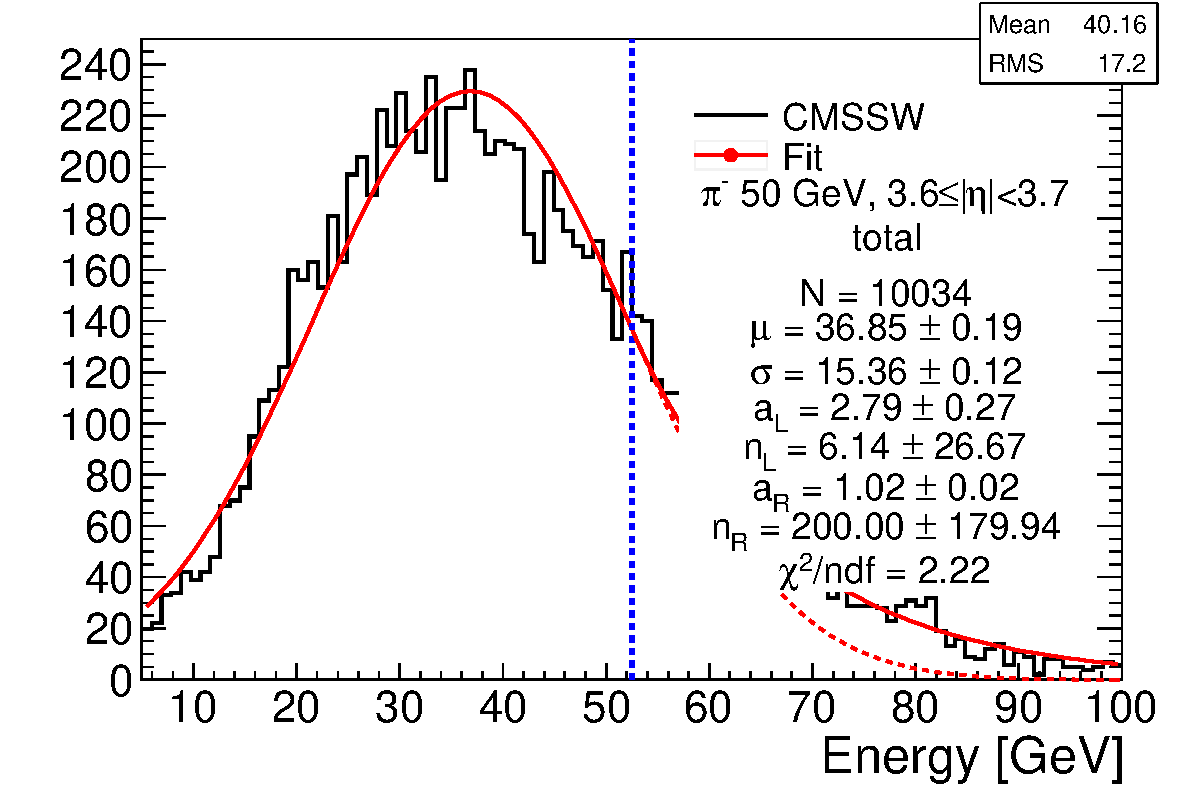
\includegraphics[width=0.49\textwidth]{figures/pion_response_tot_cballD_50gev_ieta37.pdf}
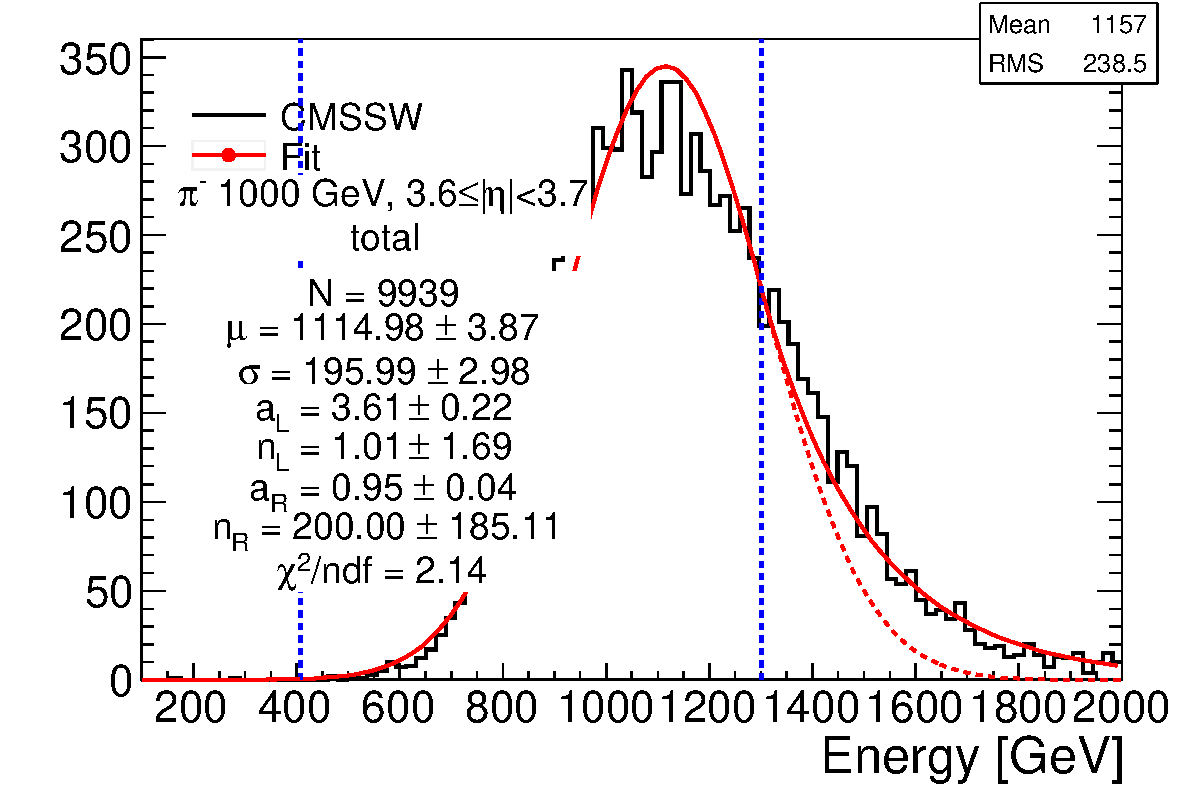
\includegraphics[width=0.49\textwidth]{figures/pion_response_tot_cballD_1000gev_ieta37.pdf}
\caption{Examples of double-sided Crystal Ball fits to simulated pion energy distributions in the HF. Medium (left) and high (right) energies are displayed for $\eta$ ranges in the HF. The blue dotted lines show the locations of the transition from the Gaussian core to the power-law tails, and the red dotted lines show a continuation of the Gaussian core for comparison to the power-law tails.}
\label{fig:cballD-fits-HF}
\end{center}
\end{figure}

Samples of \ttbar events were used to validate this new hadronic response tuning against the full simulation. A few of the validation plots, comparing the performance of both the old tuning and the new tuning to the full simulation, are shown in Fig. \ref{fig:cballD-relvals}. The new tuning is able to achieve comparable performance to the old tuning, without the use of any ad-hoc correction factors.

%figure: relvals
\begin{figure}[hbtp]
\begin{center}
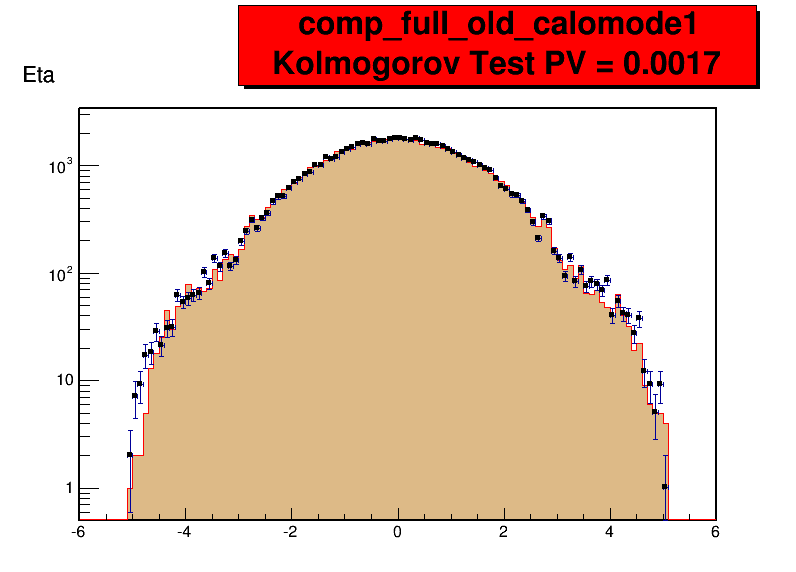
\includegraphics[width=0.49\textwidth]{figures/Eta_full_vs_fast_old.png}
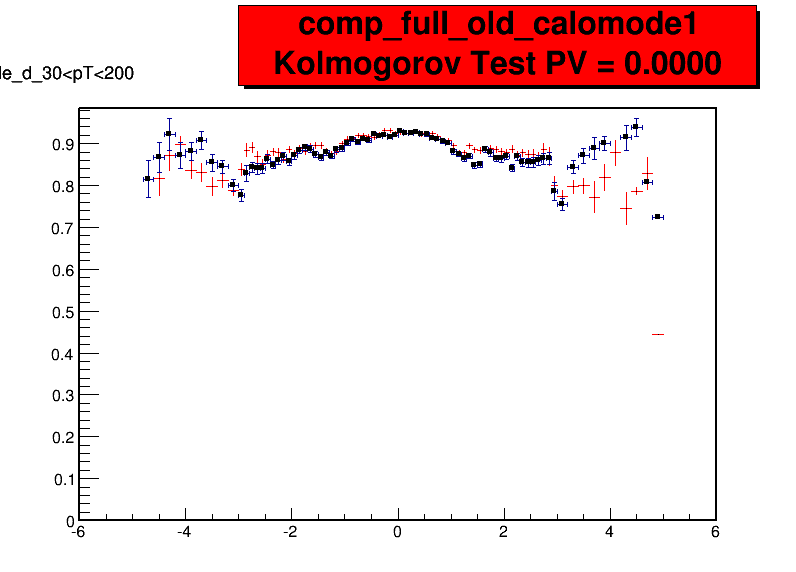
\includegraphics[width=0.49\textwidth]{figures/pTScale_d_30_pT_200_full_vs_fast_old.png}
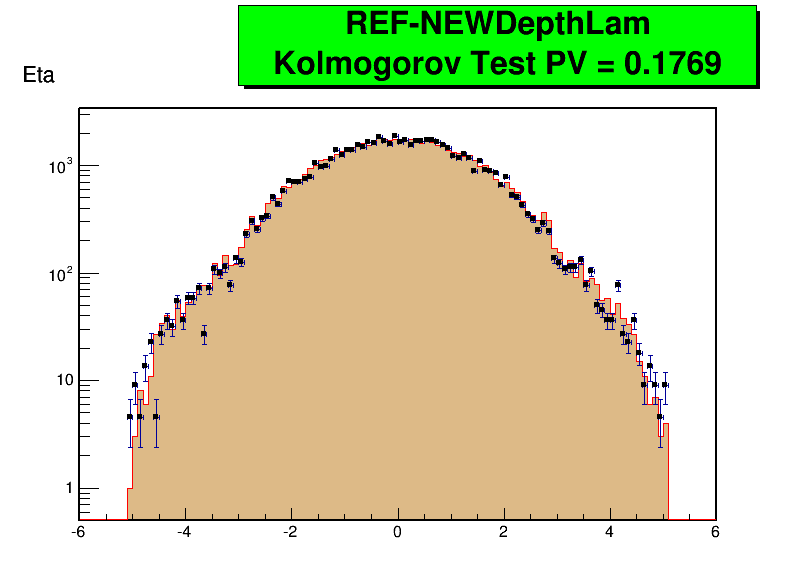
\includegraphics[width=0.49\textwidth]{figures/Eta_full_vs_fast_new.png}
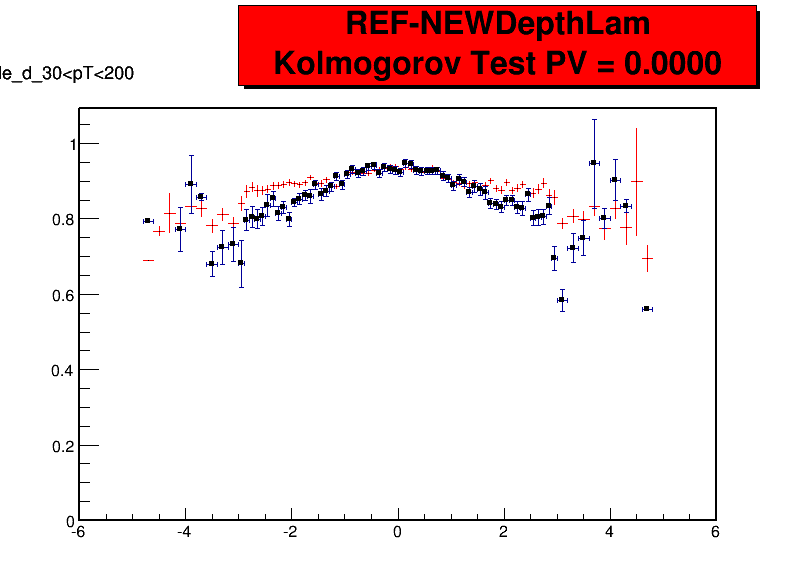
\includegraphics[width=0.49\textwidth]{figures/pTScale_d_30_pT_200_full_vs_fast_new.png}
\caption{Plots of the $\eta$ distribution (left) and \pt response vs. $\eta$ (right) for PF jets in \ttbar samples, comparing the full simulation (red) to the fast simulation (black) with the old hadronic response tuning (top) and the new hadronic response tuning (bottom).}
\label{fig:cballD-relvals}
\end{center}
\end{figure}

%Results from Reza could be added here
\subsection{MIP Fraction in Hadronic Showers}

In the CMS hadronic shower fast simulation, the shower starting depth $s$ is simulated using an exponential distribution. This distribution can be treated as a PDF integrated to find the CDF for inversion sampling, where $x \in [0,1]$ is a uniformly distributed random number:
\begin{align}
f(s) &= e^{-s}\\
F(s) &= \int_{0}^{s} f(s^{\prime})ds^{\prime} = 1 - e^{-s}\\
x \equiv F(s) &\rightarrow F^{-1}(x) = -\text{ln}(1-x) = \text{ln}\left(\frac{1}{x}\right) = s
\end{align}
In the last step, the fact that $x$ is a uniformly distributed random number in $[0,1]$ is used to take $(1-x) \rightarrow x$.

The condition which decides if the shower will start in the ECAL is based on a comparison between the depth of the ECAL $d_{\text{ecal}}$ and the starting depth $s$. If the shower does not start in the ECAL, the incident hadron is considered to be a minimum ionizing particle (MIP) in the ECAL.
\begin{align}
\frac{d_{\text{ecal}}-s}{d_{\text{ecal}}} > 0.1 &\\
0.9 d_{\text{ecal}} > s~&\text{(for pion showers starting in ECAL)} \\
0.9 d_{\text{ecal}} \leq s~&\text{(for pions which are MIPs in ECAL)} \\
d \equiv 0.9 d_{\text{ecal}}~&\text{(the minimum starting distance for MIPs)}
\end{align}

Since $f(s)$ is a probability distribution, it has area 1 in $[0,\infty]$. The area for $s = d..\infty$, when $s \geq d$, is equal to the probability $p$ that the particle is a MIP. In order to solve this problem, the distribution must be transformed to introduce a free parameter:
\begin{align}
f(s,\lambda) &= \lambda e^{-\lambda s}\\
s &= \frac{1}{\lambda}\text{ln}\left(\frac{1}{x}\right)
\end{align}

Now the integral can be solved to require the correct MIP fraction:
\begin{align}
p = \int_{d}^{\infty} ds \lambda e^{-\lambda s} &= e^{-\lambda d}\\
\rightarrow \lambda &= \frac{1}{d}\text{ln}\left(\frac{1}{p}\right)
\end{align}

Since $d$ is determined by detector geometry, for any $p \in (0,1)$, $\lambda$ can be found to ensure the correct MIP fraction. The final result is just a scaling by $1/\lambda$ of the original equation for randomly generating $s$ from the uniform random number $x$. In practice, $p$ can be determined from the full simulation as a function of the incident particle energy and $\eta$. The pion samples used for the new hadronic response tuning were also used to determine these probability values, classifying a particle as a MIP if it deposits less than 0.8\GeV of energy in the ECAL. Figure \ref{fig:mippct} shows two examples of the MIP fraction versus energy. Figure \ref{fig:allmippct} shows the MIP fractions for the entire energy and $\eta$ range of the calorimeter system, including linear interpolation for intermediate energies. For energies outside the simulated range, the first or last values are used instead of extrapolating, as extrapolating could produce $p \leq 0$ or $p \geq 1$, which would create unphysical values $\lambda \not\in (0,\infty)$.

\begin{figure}[hbtp]
\begin{center}
\includegraphics[width=0.49\textwidth]{figures/fs_plot_mip_ieta1.pdf}
\includegraphics[width=0.49\textwidth]{figures/fs_plot_mip_ieta20.pdf}
\caption{Plots of MIP percentage vs. energy for $i\eta = 1$ (in the barrel) and $i\eta = 20$ (in the endcap).}
\label{fig:mippct}
\end{center}
\end{figure}

\begin{figure}[hbtp]
\begin{center}
\includegraphics[width=0.95\textwidth]{figures/all_mip_interp.pdf}
\caption{Plots of MIP percentage vs. energy and $\eta$ for the entire calorimeter system.}
\label{fig:allmippct}
\end{center}
\end{figure}

Modeling the MIP fraction correctly in the fast simulation is one step toward using more precise response tuning by fitting separate distributions for MIP and non-MIP pions. This option is available in the fast simulation, but disabled by default. Another step is needed to complete the implementation of this option. Currently, when the hadronic shower fast simulation decides that a particle is a MIP in the ECAL, that particle deposits zero energy in the ECAL. However, this is not physically accurate; the MIP particle should actually deposit some small but non-zero amount of energy. Fixing this in the fast simulation is a difficult proposition, due to the structure of the algorithm for simulating shower energy fluctuations and the use of response smearing factors after the shower simulation.

%Also, remember that there is another section "MIP Energy in Hadronic Fast Simulation"
%but this is only a proposal, not actually implemented, so not included here (yet)

\section{Dose Rate Effects}

\subsection{Dose Rate Effect Models}

\subsection{Scintillator Radiation Damage Studies}